% ============================================================
% ch4_implementation.tex
% ANSpect O-EMA · MS Thesis · UTD Electrical Engineering
% \input target — no \documentclass or \begin{document}
% STATUS: NDA-IMPL GATED — see NDA_SCOPE.md
%         Section 4.8 OPEN — all others require handoff + NDA CLEAR
% v1.0  01-Sep-2026  Split from chapters.tex
% ============================================================

% ============================================================
% CHAPTER 4 — IMPLEMENTATION
% STATUS: NDA-IMPL — CHAPTER GATED
%
% GATE REQUIREMENTS (all must be met before any section drafts):
%   1. NDA CLEAR: IMPL [section] received for that section
%   2. Handoff file for that module uploaded in current session
%   3. Content sourced exclusively from handoff file
%   4. nda scrub run on all output before delivery
%
% EXCEPTION: Section 4.8 (Test and Measurement) — OPEN
%   4.8.1 H-Thunder-1 — public product spec
%   4.8.2 HDHomeRun    — public product
%   4.8.3 Spectrum analysis — general methodology
% ============================================================

\chapter{Implementation}
\label{ch:implementation}
% [NDA-IMPL] — chapter-level gate active
% TODO: Chapter intro paragraph — structural overview only
%   - High-level system block: PS + PL + RFDC + RF front-end
%   - No architecture detail until NDA CLEAR: IMPL [4.1] received
%   - Reference PYNQ framework existence (no internals)
 
% ------------------------------------------------------------
\section{System Architecture Overview}
\label{sec:sys_arch}
% [NDA-IMPL] — BLOCKED
% TODO: Draft requires NDA CLEAR: IMPL [4.1] + handoff upload
%   - Top-level system diagram
%   - PS/PL partition overview
%   - Data flow: UDP RX → TX chain → DAC → RF → ADC → RX chain → output
%   - No AXI register map, no overlay internals without clearance
\clearpage  
% ------------------------------------------------------------
\section{Processing System}
\label{sec:ps}
% [NDA-IMPL] — BLOCKED
% TODO: Draft requires NDA CLEAR: IMPL [4.2] + handoff upload
%   - PS subsystem structural overview only
%   - No Python driver detail, no DMA control code without clearance

\subsection{UDP/GigE RX}
\label{subsec:ps_udp_rx}
% [NDA-IMPL] — BLOCKED (PS-01)
% TODO: Requires NDA CLEAR: IMPL [4.2.1] + handoff for PS-01

\subsection{TX Chain}
\label{subsec:ps_tx_chain}
% [NDA-IMPL] — BLOCKED (PS-02)
% TODO: Requires NDA CLEAR: IMPL [4.2.2] + handoff for PS-02

\subsection{DMA Control}
\label{subsec:ps_dma_control}
% [NDA-IMPL] — BLOCKED (PS-03, PS-05)
% TODO: Requires NDA CLEAR: IMPL [4.2.3] + handoff for PS-03/PS-05
\clearpage  
% ------------------------------------------------------------
\section{Programmable Logic: TX Chain}
\label{sec:pl_tx}
% [NDA-IMPL] — BLOCKED
% TODO: Section intro requires NDA CLEAR: IMPL [4.3] + handoff
%   - PL-01 through PL-12 — one subsection each
%   - PL-10 (SD-FEC LDPC) also touches [NDA-ALGO] boundary —
%     see subsection note below

\subsection{PL-01: AXI DMA MM2S}
\label{subsec:pl01}
% [NDA-IMPL] — BLOCKED
% TODO: Requires NDA CLEAR: IMPL [4.3.1] + handoff for PL-01

% ============================================================
% CH-4.3.2  PL-02: TRANSPORT_FRAMING
% Source : PL-02_TRANSPORT_FRAMING_handoff.md v2.1  09-Jul-2026
%          transport_framing.sv v2.1
% NDA CLEAR: IMPL [4.3] — received
% Preflight : CH-4.3.2 [PL-02] — PASS  21-Oct-2026
%   IMG-1 [x]  IMG-2 [x]  IMG-3 [OMITTED — author]  IMG-4 [x]  IMG-5 [x]
% Expanded  : 21-Oct-2026
% Template  : CARRY_FORWARD.md §1–§8 v1.2
% ============================================================

\subsection{PL-02: Transport Framing}
\label{subsec:pl02}

% ------------------------------------------------------------------
% §1  OVERVIEW
% ------------------------------------------------------------------

The transport framing module (PL-02) implements the \ac{mpegts} packet
framing stage of the J.83B Annex~B transmit chain, specified in
\S\,B.4 of the standard~\cite{ITU_J83}.
The algorithmic background for this stage is described in
Section~\ref{sec:j83b_standard}; this section covers its hardware
realization.
The module is hand-coded SystemVerilog (\texttt{transport\_framing.sv},
revision~v2.1), operates as an \ac{axi}4-Stream slave-to-master pair at
the 250\,MHz \ac{pl} fabric clock, and carries a testbench status of
TB-PASS (174{,}777 checks, 0 failures).
Its position in the transmit chain is shown in
Figure~\ref{fig:pl02_pipeline}.

% [ALT: Block diagram showing three rectangular blocks in a horizontal
%       row. Left block: PL-01 AXI DMA MM2S. Centre block (highlighted
%       green): PL-02 TRANSPORT_FRAMING. Right block: PL-03 RS_ENC.
%       Arrows between blocks are labeled 8-bit AXI-S. A 250 MHz PL
%       clock label appears below the chain; no CDC marker is present
%       at either boundary.]
\begin{figure}[htbp]
  \centering
  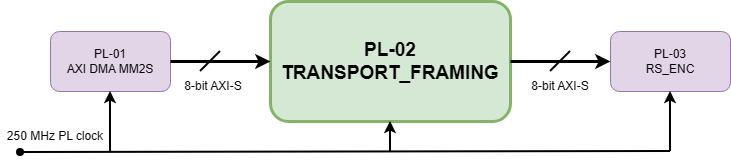
\includegraphics[width=0.85\linewidth]{figures/ch4/ch4_pl02_pipeline}
  \caption{Pipeline position of PL-02 \texttt{transport\_framing} in the
           J.83B Annex~B transmit chain.}
  \label{fig:pl02_pipeline}
\end{figure}

% ------------------------------------------------------------------
% §2  INTERFACE
% ------------------------------------------------------------------

\paragraph{Interface.}

% [ALT: Screenshot of the transport_framing IP core in Vivado IP
%       Integrator. The block is labelled transport_framing with the
%       subtitle J.83B Transport Framing (PL-02) (Pre-Production).
%       On the left side the s_axi slave interface group shows ports
%       s_axi_tdata[7:0], s_axi_tvalid, and s_axi_tready. Control
%       ports clk and rst_n appear below the interface group. On the
%       right side the m_axi master interface group shows ports
%       m_axi_tdata[7:0], m_axi_tvalid, and m_axi_tready.]
\begin{figure}[htbp]
  \centering
  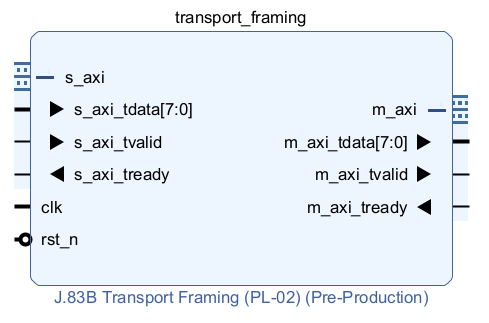
\includegraphics[width=0.55\linewidth]{figures/ch4/ch4_pl02_ip_block}
  \caption{PL-02 \texttt{transport\_framing} packaged as a Vivado \ac{ip}
           core in \ac{ip} Integrator, showing the \texttt{s\_axi} slave
           and \texttt{m\_axi} master interface groups.}
  \label{fig:pl02_ip_block}
\end{figure}

\FloatBarrier 

\begin{table}[htbp]
  \caption{PL-02 \texttt{transport\_framing} port list.}
  \label{tab:pl02_ports}
  \centering
  \begin{tabular}{llcll}
    \hline
    Port                    & Dir  & Width & Protocol              & Description \\
    \hline
    \texttt{clk}            & in   & 1     & Clock                 & 250\,MHz \ac{pl} fabric clock \\[2pt]
    \texttt{rst\_n}         & in   & 1     & Reset                 & Synchronous active-low \\[2pt]
    \texttt{s\_axi\_tdata}  & in   & 8     & \ac{axi}4-Stream slave  & \ac{mpegts} byte stream from PL-01 \\[2pt]
    \texttt{s\_axi\_tvalid} & in   & 1     & \ac{axi}4-Stream slave  & Upstream data valid \\[2pt]
    \texttt{s\_axi\_tready} & out  & 1     & \ac{axi}4-Stream slave  & Upstream backpressure \\[2pt]
    \texttt{m\_axi\_tdata}  & out  & 8     & \ac{axi}4-Stream master & Framed byte stream to PL-03 \\[2pt]
    \texttt{m\_axi\_tvalid} & out  & 1     & \ac{axi}4-Stream master & Downstream data valid \\[2pt]
    \texttt{m\_axi\_tready} & in   & 1     & \ac{axi}4-Stream master & Downstream backpressure \\
    \hline
  \end{tabular}
\end{table}

% ------------------------------------------------------------------
% §3  RTL ARCHITECTURE
% ------------------------------------------------------------------

\paragraph{RTL Architecture.}
% [FIGURE OMITTED: datapath diagram figures/ch4_pl02_datapath — omitted by author]

The module is organized as a two-block combinational datapath driving a
set of registered state elements, with an output mux controlled by the
\ac{fsm} state described in the following section.
Registered state consists of five elements: the 2-bit \ac{fsm} state,
an 8-bit byte counter (\texttt{byte\_cnt}), three 8-bit \ac{lfsr}
registers (\texttt{r1}, \texttt{r2}, \texttt{r3}), an 8-bit
\texttt{first7} capture register, and an 8-bit \texttt{checksum}
register.
Registers \texttt{r2} and \texttt{r3} are initialized to
\texttt{0x00} per the J.83B §B.4 specification and are never
subsequently updated~\cite{ITU_J83}; they are retained in the
\ac{rtl} for algorithmic traceability.

The \texttt{ph1\_lfsr\_chain} block implements the 8-step bit-serial
Phase~1 \ac{lfsr} computation as a fully unrolled
\texttt{always\_comb} loop, producing \texttt{r1\_ph1\_next} and
\texttt{first7\_next} every clock cycle.
Results are latched into \texttt{r1} and \texttt{first7} only on an
input handshake event while in \texttt{PH\_ONE}.
The \texttt{ph2\_lookup\_and\_drain} block executes unconditionally every
cycle, computing both the Phase~2 table-lookup result
(\texttt{r1\_ph2\_next}) and the full 8-step Phase~3 drain chain
(\texttt{checksum\_next}).
The drain result is latched into the \texttt{checksum} register only when
\texttt{byte\_cnt}~$\geq 187$ in \texttt{PH\_TWO}.
Running the drain chain unconditionally on every cycle simplifies control
logic at the cost of switching activity on the 186 non-drain cycles per
packet; this is a deferred power optimization with no functional impact.

\texttt{m\_axi\_tdata} is driven by a state-selected combinational mux:
it carries \texttt{checksum} in \texttt{PH\_THREE} and passes
\texttt{s\_axi\_tdata} through combinationally in all other states.
\texttt{s\_axi\_tready} is a priority conditional assignment that returns
\texttt{0} in \texttt{PH\_THREE}, \texttt{1} in \texttt{PH\_SYNC}, and
\texttt{m\_axi\_tready} otherwise.
Post-implementation timing analysis confirmed that the combinational
\texttt{s\_axi\_tready} path through \texttt{m\_axi\_tready} meets the
250\,MHz constraint with a worst negative slack of
$+2.687$\,ns~(Table~\ref{tab:pl02_timing}), so no registered pipeline
cut was introduced.

% ------------------------------------------------------------------
% §4  FSM
% ------------------------------------------------------------------

\paragraph{FSM.}
The four-state \ac{fsm} maps directly onto the three-phase checksum
computation.
Figure~\ref{fig:pl02_fsm} shows the state transition diagram;
Table~\ref{tab:pl02_fsm} gives the handshake signal values per state.

% [ALT: State transition diagram with four circular states. PH_SYNC(0)
%       is at top-left, PH_ONE(1) at top-right, PH_TWO(2) at
%       bottom-right, and PH_THREE(3) at bottom-left, arranged in a
%       clockwise cycle. Transition arcs are labeled: PH_SYNC to
%       PH_ONE on input_hs and tdata==0x47; PH_SYNC self-loop on
%       input_hs and tdata!=0x47; PH_ONE to PH_TWO on input_hs;
%       PH_TWO self-loop on input_hs and byte_cnt<187; PH_TWO to
%       PH_THREE on input_hs and byte_cnt>=187; PH_THREE to PH_SYNC
%       on output_hs. Each state bubble shows its s_tready and
%       m_tvalid values. A reset arc enters PH_SYNC from above.]
\begin{figure}[htbp]
  \centering
  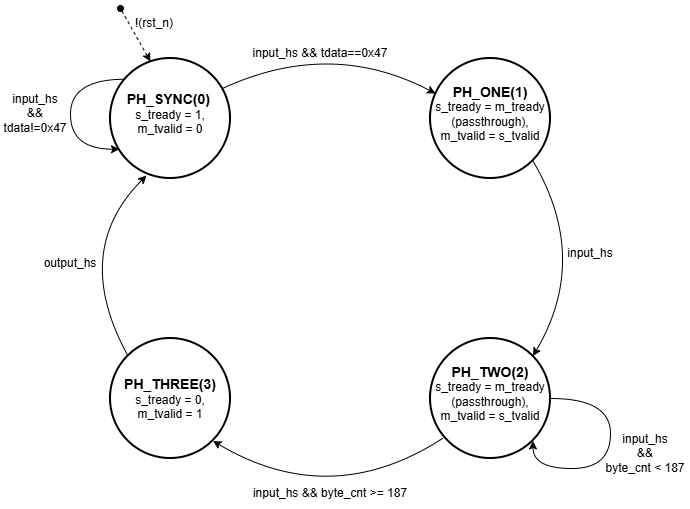
\includegraphics[width=0.72\linewidth]{figures/ch4/ch4_pl02_fsm}
  \caption{PL-02 \ac{fsm} state transition diagram.
           \texttt{input\_hs}:\ \texttt{s\_axi\_tvalid \&\ s\_axi\_tready};
           \texttt{output\_hs}:\ \texttt{m\_axi\_tvalid \&\ m\_axi\_tready}.}
  \label{fig:pl02_fsm}
\end{figure}

\FloatBarrier

\begin{table}[htbp]
  \caption{PL-02 \ac{fsm} handshake signal matrix.}
  \label{tab:pl02_fsm}
  \centering
  \begin{tabular}{llll}
    \hline
    State              & \texttt{s\_axi\_tready}   & \texttt{m\_axi\_tvalid}   & Notes \\
    \hline
    \texttt{PH\_SYNC}  & \texttt{1} (forced)       & \texttt{0}                & Sync hunt; no output \\[2pt]
    \texttt{PH\_ONE}   & \texttt{m\_axi\_tready}   & \texttt{s\_axi\_tvalid}   & Phase~1; backpressure passthrough \\[2pt]
    \texttt{PH\_TWO}   & \texttt{m\_axi\_tready}   & \texttt{s\_axi\_tvalid}   & Phase~2; backpressure passthrough \\[2pt]
    \texttt{PH\_THREE} & \texttt{0} (forced)       & \texttt{1} (forced)       & Input stalled; checksum byte driven \\
    \hline
  \end{tabular}
\end{table}

In \texttt{PH\_SYNC}, \texttt{s\_axi\_tready} is forced high
unconditionally, decoupled from \texttt{m\_axi\_tready} (revision~v2.1).
This decoupling resolves a cold-boot deadlock in which the module waited
for \ac{rs} encoder readiness before accepting the first \texttt{0x47}
byte, while the \ac{rs} encoder simultaneously awaited valid input data —
a circular stall with no external resolution.
Since \texttt{PH\_SYNC} produces no output (\texttt{m\_axi\_tvalid}~$= 0$),
downstream readiness is irrelevant in this state and the decoupling is
unconditional.

% ------------------------------------------------------------------
% §5  MEMORY RESOURCES
% ------------------------------------------------------------------

\paragraph{Memory Resources.}
Two 256-entry read-only tables support the Phase~2 and Phase~3 checksum
computation.
Both are pre-computed offline using the ANSpect J.83B reference
implementation~\cite{ITU_J83}, with the generator script
\texttt{write\_transport\_framing\_roms.m} extracting and writing
the tables to \texttt{.mem} format, and loaded at simulation time via \texttt{\$readmemh}.
The \texttt{rom\_style = "distributed"} synthesis attribute directs
Vivado~2024.2 to constant-fold both tables into combinational \ac{lut}
logic; no \ac{bram} primitive is inferred.
Table~\ref{tab:pl02_roms} lists the ROM parameters.

\begin{table}[htbp]
  \caption{PL-02 ROM configuration.}
  \label{tab:pl02_roms}
  \centering
  \small
  \begin{tabular}{llllcc}
    \hline
    ROM                  & Depth$\times$Width  & Synthesis    & Content                         & Verified & Source file \\
    \hline
    \texttt{CRC\_ROM}    & $256 \times 8$      & Distributed  & Phase~2 CRC table (\texttt{pCrc[]})    & 256/256  & \texttt{crc\_rom.mem} \\[2pt]
    \texttt{BITREV\_ROM} & $256 \times 8$      & Distributed  & Bit-reversal table (\texttt{pBit[]})   & 256/256  & \texttt{bitrev\_rom.mem} \\
    \hline
    \multicolumn{6}{l}{\small Combined \ac{lut} cost: 64 \acp{lut} total (both ROMs + all RTL logic; constant-folded, Vivado~2024.2)} \\
    \hline
  \end{tabular}
\end{table}

% ------------------------------------------------------------------
% §6  INTERFACE CONTRACT
% ------------------------------------------------------------------

\paragraph{Interface Contract.}

\textit{Upstream (\texttt{s\_axi\_*}, from PL-01 \ac{axi} \ac{dma} MM2S):}
\begin{itemize}
  \item Every packet must begin with the \ac{mpegts} sync byte
        \texttt{0x47}~\cite{ITU_J83}.
        Bytes received before the first \texttt{0x47} are consumed and
        discarded in \texttt{PH\_SYNC}.
  \item \texttt{s\_axi\_tready} is state-dependent: forced high in
        \texttt{PH\_SYNC}; equal to \texttt{m\_axi\_tready} in
        \texttt{PH\_ONE} and \texttt{PH\_TWO}; forced low in
        \texttt{PH\_THREE}.
        The upstream source must tolerate 1-cycle
        \texttt{s\_axi\_tready} deassertions at each
        \texttt{PH\_SYNC}$\to$\texttt{PH\_ONE} packet boundary
        (confirmed in integration testbench: 250~deassertions
        in a 250-packet transfer).
  \item No \texttt{tlast} signal is used.
\end{itemize}

\textit{Downstream (\texttt{m\_axi\_*}, to PL-03 \ac{rs} encoder):}
\begin{itemize}
  \item Exactly 188 bytes are emitted per input packet:
        \texttt{payload[0..186]} followed by one checksum byte.
        The \texttt{0x47} sync byte is consumed and not forwarded.
  \item \texttt{m\_axi\_tvalid} is suppressed during \texttt{PH\_SYNC},
        preventing spurious transfers to the \ac{rs} encoder during
        sync hunt.
        In \texttt{PH\_THREE}, \texttt{m\_axi\_tvalid} is forced high
        regardless of upstream state.
  \item Back-to-back packet operation is supported with no idle gap:
        the \texttt{PH\_THREE}$\to$\texttt{PH\_SYNC} transition occurs
        on the output handshake of the checksum byte.
  \item Checksum drain latency is 1~clock cycle: the checksum byte
        appears at the module output within one clock of the final
        payload byte being accepted (confirmed in integration testbench).
  \item No \texttt{tlast} signal is generated.
\end{itemize}

The output frame structure for one \ac{mpegts} packet is illustrated in
Figure~\ref{fig:pl02_packet}.

% [ALT: Packet diagram showing one 188-byte MPEG-TS output packet on
%       the AXI-Stream bus. A grey box on the left is labeled MPTS
%       sync byte 0x47 consumed by PL-02. A yellow box spanning 187
%       bytes is labeled PAYLOAD[0..186] and shows individual cells
%       Byte-0, Byte-1, Byte-4, ellipsis, Byte-185, Byte-186. A red
%       box on the right spanning 1 byte is labeled CHECKSUM 1-byte
%       and contains Byte-0. Below the diagram: tvalid=0 during
%       PH_SYNC sync byte gap; tvalid=1 payload region; tvalid=1
%       forced PH_THREE checksum; tlast not used.]
\begin{figure}[htbp]
  \centering
  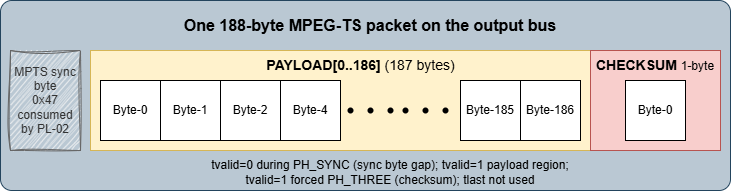
\includegraphics[width=0.88\linewidth]{figures/ch4/ch4_pl02_packet}
  \caption{PL-02 output frame structure: one reframed 188-byte
           \ac{mpegts} packet on the downstream \ac{axi}4-Stream bus.
           The \texttt{0x47} sync byte is consumed; the parity checksum
           occupies position~187~\cite{ITU_J83}.}
  \label{fig:pl02_packet}
\end{figure}

\FloatBarrier

% ------------------------------------------------------------------
% §7  RESOURCE UTILIZATION AND TIMING
% ------------------------------------------------------------------

\paragraph{Resource Utilization and Timing.}

\begin{table}[htbp]
  \caption{PL-02 post-implementation resource utilization
           (\texttt{xczu48dr-ffvg1517-2-e}, speed-grade~$-2$
           PRODUCTION, Vivado~2024.2, 21~Oct~2026).}
  \label{tab:pl02_resources}
  \centering
  \begin{tabular}{lrrl}
    \hline
    Resource     & Used & Available   & Utilization \\
    \hline
    \ac{lut6}    &  64  & 425{,}280   & 0.02\%      \\[2pt]
    \ac{ff}      &  33  & 850{,}560   & $<0.01$\%   \\[2pt]
    \ac{bram}    &   0  & 1{,}080     & 0.00\%      \\[2pt]
    \ac{dsp}     &   0  & 4{,}272     & 0.00\%      \\[2pt]
    UltraRAM     &   0  & 80          & 0.00\%      \\
    \hline
  \end{tabular}
\end{table}

\begin{table}[htbp]
  \caption{PL-02 post-implementation timing summary
           (\texttt{xczu48dr-ffvg1517-2-e}, speed-grade~$-2$
           PRODUCTION, Vivado~2024.2, 21~Oct~2026).}
  \label{tab:pl02_timing}
  \centering
  \begin{tabular}{lll}
    \hline
    Metric                 & 250\,MHz           & 100\,MHz           \\
    \hline
    WNS, setup             & $+2.687$\,ns (MET) & $+8.268$\,ns (MET) \\[2pt]
    WHS, hold              & $+0.043$\,ns (MET) & $+0.047$\,ns (MET) \\[2pt]
    Est.\ $F_{\max}$       & $\geq 372$\,MHz    & $\geq 545$\,MHz    \\[2pt]
    Failing endpoints      & 0                  & 0                  \\
    \hline
  \end{tabular}
\end{table}

\FloatBarrier

% ------------------------------------------------------------------
% §8  VERIFICATION
% ------------------------------------------------------------------

\paragraph{Verification.}

\textit{Simulation.}
Unit-level verification used a golden vector sweep of 250~\ac{mpegts}
packets against the \texttt{j83b\_transport\_framing.m} MATLAB
reference model at four upstream throttle configurations, an independent
bit-serial software model comparison across 500~randomized packets, and
adversarial payload patterns including all-zero, all-\texttt{0xFF},
alternating, and \texttt{0x47}-embedded bytes.
All 512~\ac{rom} table entries were verified against the generator
output with zero mismatches.
\ac{axi}4-Stream \ac{sva} checks confirmed no X-propagation on valid
and data stability under backpressure; \ac{fsm} reset recovery was
confirmed at all four states.

Integration testing in the PL-02$\to$PL-04 chain verified 1-cycle
checksum drain latency, zero spurious sync transitions with an
all-\texttt{0x47} adversarial payload across 47{,}000~bytes, and
deterministic checksum \texttt{0x67} for all-zero payload across
250~packets.
End-to-end testing in the PL-02$\to$PL-06 chain confirmed
8{,}304/8{,}304 trellis groups bit-exact against the stage~5 golden
reference with zero \ac{sva} fires.

\textit{Hardware.}

\begin{table}[htbp]
  \caption{PL-02 hardware validation summary.}
  \label{tab:pl02_hw}
  \centering
  \begin{tabular}{p{3.2cm}lp{4.5cm}p{3.2cm}l}
    \hline
    Bitfile & Clock & Method & Result & Date \\
    \hline
    \path{pl_2_6.bit}\\(PL-02$\to$PL-06 chain)
      & 100\,MHz
      & PYNQ \ac{dma} loopback~\cite{PYNQ_DOC}; output compared
        to \path{stage5_framesync_bits.bin}
      & 8{,}304/8{,}304 groups bit-exact;
        4/4 \ac{fec} frames PASS
      & 28-Jul-2026 \\
    \hline
  \end{tabular}
\end{table}

Board validation of PL-02 was performed indirectly as part of the
PL-02$\to$PL-06 transmit chain.
Bit-exact agreement at the PL-06 output confirms correct operation of all
intervening modules including PL-02.
The bitfile was evaluated at 100\,MHz; production operation targets
250\,MHz, which post-implementation analysis confirms meets timing with
$F_{\max} \geq 372$\,MHz~(Table~\ref{tab:pl02_timing}).

%\clearpage

% ============================================================
% CH-4.3.3  PL-03: RS_ENC
% Source : PL-03_RS_ENC_handoff.md v2.0  09-Jul-2026
%          rs_enc.sv v2.0 / gf_mul_rom.sv / main.m
% NDA CLEAR: IMPL [4.3] — received
% Preflight : CH-4.3.3 [PL-03] — PASS  22-Oct-2026
%   IMG-1 [x]  IMG-2 [x]  IMG-3 [OMITTED — author]  IMG-4 [x]  IMG-5 [x]
% Expanded  : 22-Oct-2026
% Template  : CARRY_FORWARD.md §1–§8 v1.2
% ROM attribution: ANSpect J.83B reference implementation
% ============================================================

\subsection{PL-03: Reed-Solomon Encoder}
\label{subsec:pl03}

% ------------------------------------------------------------------
% §1  OVERVIEW
% ------------------------------------------------------------------

The Reed-Solomon encoder module (PL-03) implements the J.83B Annex~B
$(128,\,122)$ extended \ac{rs} encoding stage over $\mathrm{GF}(2^7)$,
specified in \S\,B.5.1 of the standard~\cite{ITU_J83}.
The algorithmic definition of this code — field arithmetic, generator
polynomial, parity computation, and extended symbol derivation — is
presented in Section~\ref{sec:rs_encoding}; this section describes
its hardware realization.
The module is hand-coded SystemVerilog (\texttt{rs\_enc.sv},
revision~v2.0), operates as an \ac{axi}4-Stream slave-to-master pair
at the 250\,MHz \ac{pl} fabric clock, and carries a testbench status
of TB-PASS (49{,}570 checks, 0 failures).
Figure~\ref{fig:pl03_pipeline} shows its position in the transmit chain,
receiving framed bytes from the transport framing module (PL-02) and
forwarding $(128,\,122)$ coded blocks to the convolutional interleaver
(PL-04).

% [ALT: Block diagram showing three rectangular blocks in a horizontal
%       row. Left block: PL-02 TRANSPORT_FRAMING. Centre block
%       (highlighted green): PL-03 RS_ENC. Right block: PL-04
%       INTERLEAVER. Arrows between blocks are labeled 8-bit AXI-S.
%       A 250 MHz PL clock label appears below the chain; no CDC
%       marker is present at either boundary.]
\begin{figure}[htbp]
  \centering
  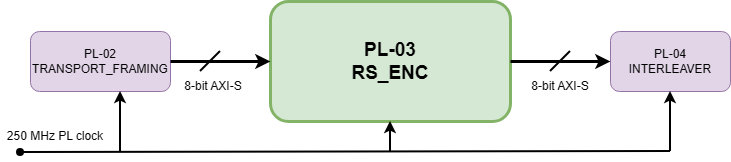
\includegraphics[width=0.65\linewidth]{figures/ch4/ch4_pl03_pipeline}
  \caption{Pipeline position of PL-03 \texttt{rs\_enc} in the
           J.83B Annex~B transmit chain.}
  \label{fig:pl03_pipeline}
\end{figure}

% ------------------------------------------------------------------
% §2  INTERFACE
% ------------------------------------------------------------------

\paragraph{Interface.}

The Vivado \ac{ip} Integrator view in Figure~\ref{fig:pl03_ip_block}
shows the packaged \texttt{rs\_enc} core with the \texttt{s\_axi} slave
interface group on the left and the \texttt{m\_axi} master interface group
on the right.
The port list is given in Table~\ref{tab:pl03_ports}.

% [ALT: Screenshot of the rs_enc IP core in Vivado IP Integrator. The
%       block is labeled rs_encoder with the subtitle J.83B RS Encoder
%       (PL-03) (Pre-Production). On the left side the s_axi slave
%       interface group shows ports s_axi_tdata[7:0], s_axi_tvalid,
%       and s_axi_tready. Control ports clk and rst_n appear below.
%       On the right side the m_axi master interface group shows ports
%       m_axi_tdata[7:0], m_axi_tvalid, and m_axi_tready.]
\begin{figure}[htbp]
  \centering
  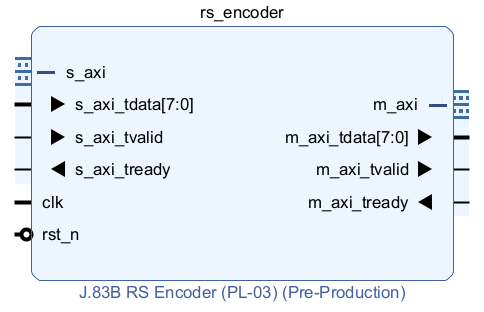
\includegraphics[width=0.35\linewidth]{figures/ch4/ch4_pl03_ip_block}
  \caption{PL-03 \texttt{rs\_enc} packaged as a Vivado \ac{ip} core
           in \ac{ip} Integrator, showing the \texttt{s\_axi} slave
           and \texttt{m\_axi} master interface groups.}
  \label{fig:pl03_ip_block}
\end{figure}

\FloatBarrier

\begin{table}[htbp]
  \caption{PL-03 \texttt{rs\_enc} port list.}
  \label{tab:pl03_ports}
  \centering
  \small
  \begin{tabular}{llcp{3.7cm}p{5.8cm}}
    \hline
    Port                    & Dir  & Width & Protocol               & Description \\
    \hline
    \texttt{clk}            & in   & 1     & Clock                  & 250\,MHz \ac{pl} fabric clock \\[2pt]
    \texttt{rst\_n}         & in   & 1     & Reset                  & Synchronous active-low \\[2pt]
    \texttt{s\_axi\_tdata}  & in   & 8     & \ac{axi}4-Stream slave & Framed byte from PL-02; bit~7 masked internally \\[2pt]
    \texttt{s\_axi\_tvalid} & in   & 1     & \ac{axi}4-Stream slave & Upstream data valid \\[2pt]
    \texttt{s\_axi\_tready} & out  & 1     & \ac{axi}4-Stream slave & Upstream backpressure \\[2pt]
    \texttt{m\_axi\_tdata}  & out  & 8     & \ac{axi}4-Stream master & \ac{rs}-encoded symbol to PL-04; bit~7 always 0 \\[2pt]
    \texttt{m\_axi\_tvalid} & out  & 1     & \ac{axi}4-Stream master & Downstream data valid \\[2pt]
    \texttt{m\_axi\_tready} & in   & 1     & \ac{axi}4-Stream master & Downstream backpressure \\
    \hline
  \end{tabular}
\end{table}

% ------------------------------------------------------------------
% §3  FSM
% ------------------------------------------------------------------

\paragraph{FSM.}

The module processes one \ac{rs} block at a time through a fixed
five-stage sequence: wait, collect, send data, send parity, send
extended symbol.
Figure~\ref{fig:pl03_fsm} shows the state diagram; each state
corresponds directly to one of these tasks.

% [ALT: State diagram with five circular states. IDLE(0) is top-left
%       with s_tready=0 and m_tvalid=0. ABSORB(1) is top-right with
%       s_tready=1 and m_tvalid=0. EMIT_INFO(2) is middle-right with
%       s_tready=0 and m_tvalid=1, annotated stalls at out_cnt==121
%       until horner_done. EMIT_PAR(3) is bottom-centre with
%       s_tready=0 and m_tvalid=1. EMIT_EXT(4) is bottom-left with
%       s_tready=0 and m_tvalid=1. A dashed reset arc enters IDLE.
%       IDLE to ABSORB: s_axi_tvalid. ABSORB self-loop: !(input_hs
%       && sym_cnt==121). ABSORB to EMIT_INFO: input_hs &&
%       sym_cnt==121. EMIT_INFO self-loop: !(output_hs &&
%       out_cnt==121 && horner_done). EMIT_INFO to EMIT_PAR:
%       output_hs && out_cnt==121 && horner_done. EMIT_PAR
%       self-loop: !(output_hs && out_cnt==4). EMIT_PAR to EMIT_EXT:
%       output_hs && out_cnt==4. EMIT_EXT to ABSORB: output_hs.]
\begin{figure}[htbp]
  \centering
  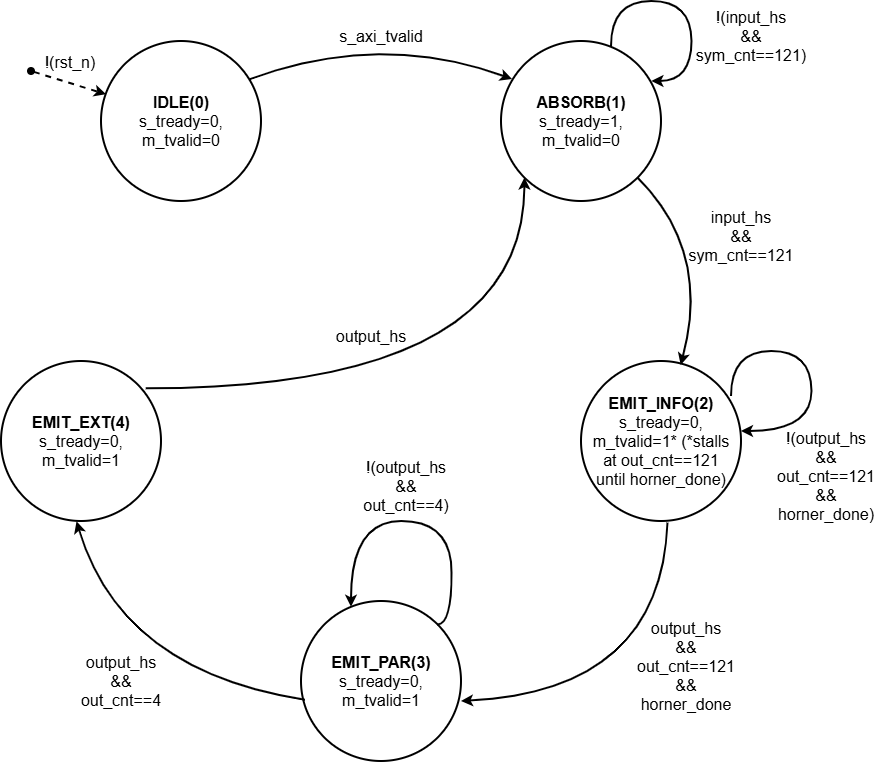
\includegraphics[width=0.70\linewidth]{figures/ch4/ch4_pl03_fsm}
  \caption{PL-03 \ac{fsm} state transition diagram.
           \texttt{input\_hs}:\ \texttt{s\_axi\_tvalid \&\ s\_axi\_tready};
           \texttt{output\_hs}:\ \texttt{m\_axi\_tvalid \&\ m\_axi\_tready}.
           The \texttt{EMIT\_INFO} state pauses output for exactly
           5~cycles at \texttt{out\_cnt}~$= 121$ while the background
           Horner computation completes.}
  \label{fig:pl03_fsm}
\end{figure}

\FloatBarrier

\texttt{IDLE} is the power-on state after reset.
The module holds \texttt{s\_axi\_tready} low and waits.
When the upstream transport framing module has a byte ready, it asserts
\texttt{s\_axi\_tvalid} and holds both \texttt{tvalid} and
\texttt{tdata} stable until the transfer is accepted — this is the
\ac{axi}4-Stream master obligation~\cite{ARM_IHI0022}.
PL-03 detects \texttt{s\_axi\_tvalid} in \texttt{IDLE} and transitions
to \texttt{ABSORB} on the next clock cycle, where \texttt{s\_axi\_tready}
rises.
The upstream byte is consumed on that same cycle when both signals are
high simultaneously.
No data is lost and no deadlock occurs: PL-02 holds its byte stable,
PL-03 raises readiness one cycle later, and the transfer completes.

\texttt{ABSORB} is the collection phase.
The module accepts the 122 input bytes one at a time, storing each
into the \texttt{cw[]} register array.
While bytes are being accepted, the five \ac{rs} parity values are
computed incrementally in the background using a $\mathrm{GF}(128)$
\ac{lfsr}~\cite{ITU_J83}; no separate encoding pass is needed.
\texttt{s\_axi\_tready} is high only in this state, so the upstream
module knows the encoder is ready to accept data.

\texttt{EMIT\_INFO} is the data forwarding phase.
The 122 original bytes are sent downstream unchanged.
Simultaneously, the module begins computing the extended symbol
$c(\alpha^6)$ in the background using Horner's method over the
complete 127-symbol codeword~\cite{ITU_J83}.
This background computation finishes just after the last info byte
is presented — specifically, 5~clock cycles after byte~121 is ready
to send.
During these 5~cycles the module pauses output (\texttt{m\_axi\_tvalid}~$= 0$)
while the computation completes.
This is the Horner stall: a short, fixed-duration gap between the
last info byte and the first parity byte, visible on the
\texttt{EMIT\_INFO} self-loop arc in Figure~\ref{fig:pl03_fsm}.

\texttt{EMIT\_PAR} sends the five computed \ac{rs} parity bytes
downstream, one per clock cycle.

\texttt{EMIT\_EXT} sends the single extended symbol byte.
On its output handshake, the module transitions directly back to
\texttt{ABSORB} — ready to accept the next block with no idle gap
and without returning through \texttt{IDLE}.

Table~\ref{tab:pl03_fsm} gives the handshake signal values in
each state.



\begin{table}[htbp]
  \caption{PL-03 \ac{fsm} state summary.}
  \label{tab:pl03_fsm}
  \centering
  \begin{tabular}{lllp{5.5cm}}
    \hline
    State               & \texttt{s\_axi\_tready} & \texttt{m\_axi\_tvalid} & Task \\
    \hline
    \texttt{IDLE}       & \texttt{0} & \texttt{0}       & Waiting for first upstream byte \\[2pt]
    \texttt{ABSORB}     & \texttt{1} & \texttt{0}       & Collecting 122 input bytes; computing RS parity in background \\[2pt]
    \texttt{EMIT\_INFO} & \texttt{0} & \texttt{1}$^{*}$ & Forwarding 122 info bytes; computing extended symbol in background ($^{*}$5-cycle pause at byte~121) \\[2pt]
    \texttt{EMIT\_PAR}  & \texttt{0} & \texttt{1}       & Sending 5 RS parity bytes \\[2pt]
    \texttt{EMIT\_EXT}  & \texttt{0} & \texttt{1}       & Sending extended symbol; transitions to \texttt{ABSORB} on completion \\
    \hline
  \end{tabular}
\end{table}

\texttt{s\_axi\_tready} is a pure combinational state decode
(\texttt{assign s\_axi\_tready = (state == ABSORB)}), with no path
from \texttt{m\_axi\_tready} to \texttt{s\_axi\_tready}.
Downstream backpressure from PL-04 does not propagate upstream to PL-02.

% ------------------------------------------------------------------
% §4  MEMORY RESOURCES
% ------------------------------------------------------------------

\paragraph{Memory Resources.}
All $\mathrm{GF}(128)$ multiplications in the \ac{lfsr} encoder and
the Horner evaluator are provided by a common sub-module,
\texttt{gf\_mul\_rom.sv}, instantiated six times.
Each instance is a $16{,}384 \times 7$-bit combinational \ac{rom}
addressed by the 14-bit concatenation $\{a[6:0],\,b[6:0]\}$,
implementing the full $128 \times 128$ $\mathrm{GF}(128)$ multiplication
table for $p(x) = x^7 + x^3 + 1$~\cite{ITU_J83}.
The \texttt{rom\_style = "distributed"} attribute produces a single-cycle
combinational read synthesized entirely into distributed \ac{lut}
logic with no \ac{bram} consumed.
The \ac{rom} content was pre-computed offline using the ANSpect J.83B
reference implementation~\cite{ITU_J83}, with \texttt{main.m} extracting
the $\mathrm{GF}(128)$ table via the \texttt{j83b\_rs\_encode('tables')}
accessor and writing it to \texttt{gf\_mul.mem}.
Table~\ref{tab:pl03_roms} lists the sub-module configuration.

\begin{table}[htbp]
  \caption{PL-03 \texttt{gf\_mul\_rom} sub-module configuration.}
  \label{tab:pl03_roms}
  \centering
  \small
  \begin{tabular}{ll}
    \hline
    Parameter        & Value \\
    \hline
    Module file      & \texttt{gf\_mul\_rom.sv} \\[2pt]
    Instances        & 6 total: \texttt{gf\_rom1}--\texttt{gf\_rom5} (\ac{lfsr} taps $G_1$--$G_5$);
                       \texttt{gf\_rom\_exp6} (Horner $\alpha^6$ step) \\[2pt]
    Depth $\times$ Width & $16{,}384 \times 7$ ($128 \times 128$ entries, row-major) \\[2pt]
    Address mapping  & $\{a[6:0],\,b[6:0]\}$ \\[2pt]
    Content          & $\mathrm{GF}(128)$ multiplication table,
                       $p(x) = x^7 + x^3 + 1$ \\[2pt]
    Synthesis        & Distributed (\texttt{rom\_style = "distributed"});
                       combinational read \\[2pt]
    Source file      & \texttt{gf\_mul.mem} (shared across all 6 instances) \\[2pt]
    Generator        & MATLAB script via ANSpect J.83B reference implementation \\[2pt]
    Verification     & 529/529 entries (all generator coefficient cross-products) \\
    \hline
  \end{tabular}
\end{table}

% ------------------------------------------------------------------
% §5  RTL ARCHITECTURE
% ------------------------------------------------------------------

\paragraph{RTL Architecture.}
% [FIGURE OMITTED: datapath diagram figures/ch4_pl03_datapath — omitted by author]

With the \ac{fsm} and its memory resources established, this section
describes how each state's task is realized in hardware.

\textit{Bit masking.}
The J.83B \ac{rs} code operates on 7-bit $\mathrm{GF}(128)$ symbols;
the 8-bit \ac{axi}4-Stream bus carries one symbol per byte with bit~7
unused~\cite{ITU_J83}.
The ANSpect implementation enforces this by masking bit~7 of
\texttt{s\_axi\_tdata} to zero before any computation,
and all output symbols are formed by the
\texttt{\{1'b0,\,cw[out\_cnt]\}} concatenation in the output mux,
hardwiring bit~7 to zero on every output byte.

\textit{\texttt{ABSORB} — LFSR encoder.}
The five \texttt{gf\_mul\_rom} instances \texttt{gf\_rom1}--\texttt{gf\_rom5}
provide the $\mathrm{GF}(128)$ multiplications for generator coefficients
$G_1\!=\!62$, $G_2\!=\!46$, $G_3\!=\!98$, $G_4\!=\!70$, $G_5\!=\!11$
($\alpha^{52}$, $\alpha^{116}$, $\alpha^{119}$, $\alpha^{61}$,
$\alpha^{15}$ respectively~\cite{ITU_J83}).
The feedback input to all five instances is gated combinationally to
zero outside \texttt{ABSORB}, suppressing spurious \ac{rom} switching
in emit states.
Each accepted symbol is simultaneously written into the 127-entry,
7-bit register array \texttt{cw[0:126]}.
On the final handshake at \texttt{sym\_cnt}~$= 121$, the five computed
parity values are snapshotted into \texttt{cw[122:126]}, completing the
127-symbol codeword used by the Horner circuit.

\textit{\texttt{EMIT\_INFO} — Horner evaluator.}
The sixth instance \texttt{gf\_rom\_exp6} computes
$\bar{c} = c(\alpha^6)$ via Horner's method over \texttt{cw[0:126]}
while info bytes stream downstream.
Each step is one $\mathrm{GF}(128)$ multiply-accumulate:
$\mathtt{horner\_acc} \leftarrow \mathrm{GF\_MUL}(\mathtt{horner\_acc},\,\alpha^6)
\oplus \mathtt{cw[horner\_cnt]}$.
After 126 steps the result is latched into \texttt{ext\_sym} and
\texttt{horner\_done} asserts, ending the 5-cycle output pause and
releasing the transition to \texttt{EMIT\_PAR}.

\textit{Register array and output mux.}
The \texttt{cw[0:126]} array of $127 \times 7 = 889$
flip-flops is the dominant register resource.
Its combinational read is implemented by Vivado as a MUXF7/MUXF8
cascade (210 and 70 cells respectively), selecting
\texttt{cw[out\_cnt]} for the output mux at the full 250\,MHz clock rate.
The \texttt{parity[0:4]} registers and \texttt{cw[122:126]} hold
identical values after the parity snapshot but are not merged
by synthesis, contributing up to 35 redundant flip-flops to the
970~\ac{ff} total reported in Table~\ref{tab:pl03_resources}.

\FloatBarrier

% ------------------------------------------------------------------
% §6  INTERFACE CONTRACT
% ------------------------------------------------------------------

\paragraph{Interface Contract.}

\textit{Upstream (\texttt{s\_axi\_*}, from PL-02 transport framing):}
\begin{itemize}
  \item Input bytes are treated as 7-bit $\mathrm{GF}(128)$ symbols;
        bit~7 is masked to zero internally and does not affect the
        encoded output~\cite{ITU_J83}.
  \item \texttt{s\_axi\_tready} is asserted only in \texttt{ABSORB};
        upstream must hold valid data stable during all emit states.
  \item After reset the module enters \texttt{IDLE} with
        \texttt{s\_axi\_tready}~$= 0$.
        The first assertion of \texttt{s\_axi\_tvalid} moves the module
        to \texttt{ABSORB} within one clock cycle.
        PL-02 presents the first framed byte after its own
        \texttt{PH\_SYNC} completes, which transitions PL-03 out of
        \texttt{IDLE} with no deadlock.
  \item No \texttt{tlast} signal is used.
\end{itemize}

\textit{Downstream (\texttt{m\_axi\_*}, to PL-04 convolutional interleaver):}
\begin{itemize}
  \item Exactly 128 symbols are emitted per 122-symbol input block:
        \texttt{info[0..121]}, \texttt{parity[0..4]}, extended symbol
        $c(\alpha^6)$.
        Bit~7 is hardwired to zero on all output symbols.
  \item A fixed 5-cycle gap (\texttt{m\_axi\_tvalid}~$= 0$) appears
        between the final info symbol at position~121 and the first
        parity symbol.
        This gap is not data-dependent; its duration is fixed at
        exactly 5~cycles.
        PL-04 must tolerate a mid-block valid deassertion at this
        position.
  \item Back-to-back RS blocks are supported:
        \texttt{EMIT\_EXT} transitions to \texttt{ABSORB} on the
        extended symbol handshake with no idle gap.
  \item No \texttt{tlast} signal is generated.
\end{itemize}

Figure~\ref{fig:pl03_packet} shows the output block structure.
The three colored regions correspond directly to the three emit
states: the yellow \texttt{info[0..121]} region covers
\texttt{EMIT\_INFO}; the pink \texttt{parity[0..4]} region covers
\texttt{EMIT\_PAR}; and the green \texttt{ext} byte covers
\texttt{EMIT\_EXT}.
The gap labeled between \texttt{info[121]} and \texttt{parity[0]}
represents the 5-cycle Horner stall during which the module holds
\texttt{m\_axi\_tvalid}~$= 0$ at the \texttt{EMIT\_INFO}$\to$\texttt{EMIT\_PAR}
boundary.
The bit-packing inset confirms that bit~7 of every output byte is
\texttt{1'b0} padding, with bits~6:0 carrying the 7-bit \ac{rs}
symbol.

% [ALT: Diagram of one 128-symbol RS output block on the AXI-Stream
%       bus. A yellow section labeled info[0..121] spans 122 bytes
%       showing cells Byte-0 through Byte-121. A pink section labeled
%       parity[0..4] spans 5 bytes. A green section labeled ext spans
%       1 byte. A note below states: Horner stall tvalid=0 5 cycles
%       between info[121] and parity[0]. An inset table shows bit
%       packing: bit[7]=1b0 padding; bit[6:0]=RS Encoded data.]
\begin{figure}[htbp]
  \centering
  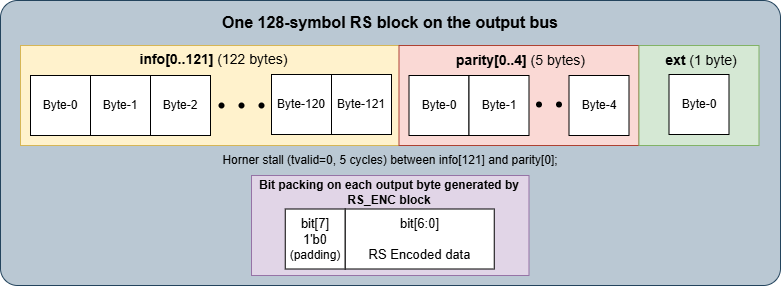
\includegraphics[width=0.88\linewidth]{figures/ch4/ch4_pl03_packet}
  \caption{PL-03 output frame structure: one 128-symbol $(128,\,122)$
           \ac{rs} block on the downstream \ac{axi}4-Stream bus.
           Bit~7 is zero-padded on all output symbols; the 5-cycle
           Horner stall between \texttt{info[121]} and
           \texttt{parity[0]} is shown at the state
           boundary~\cite{ITU_J83}.}
  \label{fig:pl03_packet}
\end{figure}

% ------------------------------------------------------------------
% §7  RESOURCE UTILIZATION AND TIMING
% ------------------------------------------------------------------

\paragraph{Resource Utilization and Timing.}
\leavevmode\par
\begin{table}[!h]
  \caption{PL-03 post-implementation resource utilization
           (\texttt{xczu48dr-ffvg1517-2-e}, speed-grade~$-2$
           PRODUCTION, Vivado~2024.2, 21~Oct~2026).}
  \label{tab:pl03_resources}
  \centering
  \begin{tabular}{lrrl}
    \hline
    Resource     & Used  & Available  & Utilization \\
    \hline
    \ac{lut6}    &  834  & 425{,}280  & 0.20\%      \\[2pt]
    \ac{ff}      &  970  & 850{,}560  & 0.11\%      \\[2pt]
    MUXF7        &  210  & N/A        & N/A          \\[2pt]
    MUXF8        &   70  & N/A        & N/A          \\[2pt]
    \ac{bram}    &    0  & 1{,}080    & 0.00\%      \\[2pt]
    \ac{dsp}     &    0  & 4{,}272    & 0.00\%      \\[2pt]
    UltraRAM     &    0  & 80         & 0.00\%      \\
    \hline
  \end{tabular}
\end{table}

\begin{table}[!h]
  \caption{PL-03 post-implementation timing summary
           (\texttt{xczu48dr-ffvg1517-2-e}, speed-grade~$-2$
           PRODUCTION, Vivado~2024.2, 21~Oct~2026).}
  \label{tab:pl03_timing}
  \centering
  \begin{tabular}{lll}
    \hline
    Metric                   & 250\,MHz           & 100\,MHz           \\
    \hline
    WNS, setup               & $+1.623$\,ns (MET) & $+6.858$\,ns (MET) \\[2pt]
    WHS, hold                & $+0.024$\,ns (MET) & $+0.047$\,ns (MET) \\[2pt]
    Est.\ $F_{\max}$         & $\geq 416$\,MHz    & $\geq 315$\,MHz    \\[2pt]
    Failing endpoints        & 0                  & 0                  \\
    \hline
  \end{tabular}
\end{table}

\FloatBarrier

% ------------------------------------------------------------------
% §8  VERIFICATION
% ------------------------------------------------------------------

\paragraph{Verification.}

\textit{Simulation.}
Unit-level verification used a 352-block golden vector sweep against the
MATLAB reference model \texttt{j83b\_rs\_encode.m}, confirming bit-exact
agreement on all 128 output symbols per block.
The extended symbol $c(\alpha^6)$ was verified independently by evaluating
the 127-symbol codeword polynomial at $\alpha^6$ via Horner's method in
software and comparing against the \ac{rtl} output.
The $\mathrm{GF}(128)$ syndrome polynomials $c(\alpha^1)$ through
$c(\alpha^5)$ were confirmed to evaluate to zero for all encoded blocks,
verifying codeword validity~\cite{ITU_J83}.
\ac{axi}4-Stream \ac{sva} checks confirmed no \texttt{m\_axi\_tvalid}
in \texttt{IDLE} or \texttt{ABSORB}, no \texttt{s\_axi\_tready} in any
emit state, and data stability under backpressure throughout.
The 5-cycle Horner stall was confirmed present on every block.
Reset recovery was verified at all five \ac{fsm} states.

Integration testing in the PL-02$\to$PL-04 chain confirmed the Horner
stall at exactly 5~cycles with zero variance across 385~RS blocks, an
RS block period of 255--256~cycles, and lossless operation under
downstream backpressure during the stall window.
End-to-end testing in the PL-02$\to$PL-06 chain confirmed
8{,}304/8{,}304 trellis groups bit-exact against the stage~5 golden
reference with zero \ac{sva} fires.

\textit{Hardware.}

\begin{table}[htbp]
  \caption{PL-03 hardware validation summary.}
  \label{tab:pl03_hw}
  \centering
  \small
  \begin{tabular}{p{3.2cm}lp{4.5cm}p{3.2cm}l}
    \hline
    Bitfile & Clock & Method & Result & Date \\
    \hline
    \path{pl_2_6.bit}\\(PL-02$\to$PL-06 chain)
      & 100\,MHz
      & PYNQ \ac{dma} loopback~\cite{PYNQ_DOC}; output compared
        to \path{stage5_framesync_bits.bin}
      & 8{,}304/8{,}304 groups bit-exact; 352~RS blocks confirmed
      & 28-Jul-2026 \\
    \hline
  \end{tabular}
\end{table}

Board validation of PL-03 was performed indirectly as part of the
PL-02$\to$PL-06 transmit chain.
Bit-exact agreement at the PL-06 output across 352~RS blocks confirms
correct parity computation and extended symbol generation.
The bitfile was evaluated at 100\,MHz; production operation targets
250\,MHz, confirmed by post-implementation timing at
$F_{\max} \geq 416$\,MHz~(Table~\ref{tab:pl03_timing}).

%\clearpage

% ============================================================
% CH-4.3.4  PL-04: INTERLEAVER
% Source : PL-04_INTERLEAVER_handoff.md v2.0  14-Jul-2026
%          interleaver.sv v2.0
% NDA CLEAR: IMPL [4.3] — received
% Preflight : CH-4.3.4 [PL-04] — PASS  22-Oct-2026
%   IMG-1 [x]  IMG-2 [x]  IMG-3 [OMITTED — author]
% Expanded  : 22-Oct-2026
% Template  : CARRY_FORWARD.md §1–§8 v1.2
%   Structure: §3 Operating Phases → §4 Memory Resources → §5 RTL Architecture
%   (per PL-03 precedent; no explicit FSM — replaced by Operating Phases)
% ============================================================

\subsection{PL-04: Convolutional Interleaver}
\label{subsec:pl04}

% ------------------------------------------------------------------
% §1  OVERVIEW
% ------------------------------------------------------------------

The convolutional interleaver module (PL-04) implements the Ramsey
Type~III convolutional interleaving stage of the J.83B Annex~B transmit
chain, specified in \S\,B.5.2 of the standard~\cite{ITU_J83}.
The algorithmic background — branch structure, delay assignment, and burst
error dispersal properties — is presented in
Section~\ref{sec:interleaving}; this section covers its hardware
realization.
The module is hand-coded SystemVerilog (\texttt{interleaver.sv},
revision~v2.0), operates as an \ac{axi}4-Stream slave-to-master pair at
the 250\,MHz \ac{pl} fabric clock, and carries a testbench status of
TB-PASS (24/24 checks, 0 failures).
Figure~\ref{fig:pl04_pipeline} shows its position in the transmit chain:
the left block is the Reed-Solomon encoder (PL-03), which supplies
\ac{rs}-encoded bytes; the right block is the randomizer (PL-05), which
receives the interleaved output.
The two 8-bit \ac{axi}4-Stream arrows indicate that the byte width is
unchanged through the stage — the interleaver reorders bytes in time but
does not alter their content or packing.

% [ALT: Block diagram showing three rectangular blocks in a horizontal row.
%       Left block: PL-03 RS_ENC. Centre block (highlighted green): PL-04
%       INTERLEAVER. Right block: PL-05 RANDOMIZER. Arrows between blocks
%       are labeled 8-bit AXI-S. A 250 MHz PL clock label appears below
%       the chain; no CDC marker at either boundary.]
\begin{figure}[htbp]
  \centering
  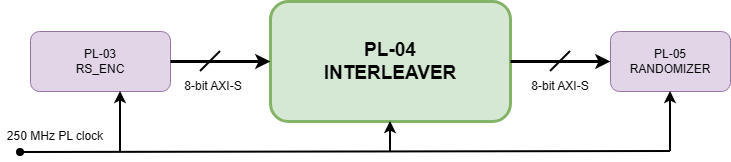
\includegraphics[width=0.85\linewidth]{figures/ch4/ch4_pl04_pipeline}
  \caption{Pipeline position of PL-04 \texttt{interleaver} in the J.83B
           Annex~B transmit chain.}
  \label{fig:pl04_pipeline}
\end{figure}

% ------------------------------------------------------------------
% §2  INTERFACE
% ------------------------------------------------------------------

\paragraph{Interface.}

Figure~\ref{fig:pl04_ip_block} shows the \texttt{interleaver} core as it
appears in the Vivado \ac{ip} Integrator block canvas.
The \texttt{s\_axi} slave group on the left receives the byte stream from
PL-03; the \texttt{m\_axi} master group on the right drives PL-05.
Two ports carry combinational signals that differ from prior modules in
the chain: \texttt{s\_axi\_tready} is a direct combinational function
of \texttt{m\_axi\_tready} and \texttt{init\_done}, and
\texttt{m\_axi\_tdata} is driven combinationally from either the \ac{bram}
read port or a passthrough register, with no registered output stage.
The port list is given in Table~\ref{tab:pl04_ports}.

% [ALT: Screenshot of the interleaver IP core in Vivado IP Integrator.
%       The block is labeled interleaver with the subtitle J.83B
%       Convolutional Interleaver (PL-04) (Pre-Production). On the left
%       side the s_axi slave interface group shows ports s_axi_tdata[7:0],
%       s_axi_tvalid, and s_axi_tready. Control ports clk and rst_n appear
%       below. On the right side the m_axi master interface group shows
%       ports m_axi_tdata[7:0], m_axi_tvalid, and m_axi_tready.]
\begin{figure}[htbp]
  \centering
  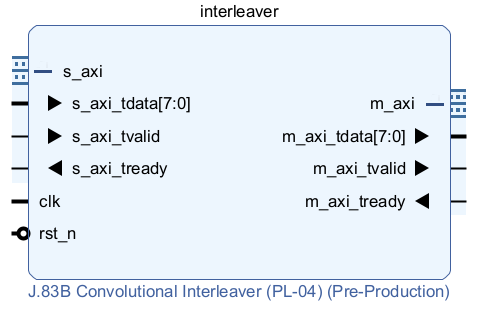
\includegraphics[width=0.55\linewidth]{figures/ch4/ch4_pl04_ip_block}
  \caption{PL-04 \texttt{interleaver} packaged as a Vivado \ac{ip} core in
           \ac{ip} Integrator, showing the \texttt{s\_axi} slave and
           \texttt{m\_axi} master interface groups.}
  \label{fig:pl04_ip_block}
\end{figure}

\FloatBarrier

\begin{table}[htbp]
  \caption{PL-04 \texttt{interleaver} port list.}
  \label{tab:pl04_ports}
  \centering
  \small
  \begin{tabular}{llcp{2.7cm}p{5.8cm}}
    \hline
    Port                    & Dir  & Width & Protocol               & Description \\
    \hline
    \texttt{clk}            & in   & 1     & Clock                  & 250\,MHz \ac{pl} fabric clock \\[2pt]
    \texttt{rst\_n}         & in   & 1     & Reset                  & Synchronous active-low \\[2pt]
    \texttt{s\_axi\_tdata}  & in   & 8     & \ac{axi}4-Stream slave & \ac{rs}-encoded byte from PL-03; bit~7 always 0 \\[2pt]
    \texttt{s\_axi\_tvalid} & in   & 1     & \ac{axi}4-Stream slave & Upstream data valid \\[2pt]
    \texttt{s\_axi\_tready} & out  & 1     & \ac{axi}4-Stream slave & Combinational: \texttt{m\_tready \&\ init\_done} \\[2pt]
    \texttt{m\_axi\_tdata}  & out  & 8     & \ac{axi}4-Stream master & Interleaved byte to PL-05; bit~7 always 0 \\[2pt]
    \texttt{m\_axi\_tvalid} & out  & 1     & \ac{axi}4-Stream master & Downstream data valid \\[2pt]
    \texttt{m\_axi\_tready} & in   & 1     & \ac{axi}4-Stream master & Downstream backpressure \\
    \hline
  \end{tabular}
\end{table}

% ------------------------------------------------------------------
% §3  OPERATING PHASES
% ------------------------------------------------------------------

\paragraph{Operating Phases.}

Unlike PL-02 and PL-03, which use explicit multi-state \acp{fsm},
PL-04 operates as a two-phase linear sequence controlled by a single
\texttt{init\_done} flag.
The two phases exist because the Ramsey Type~III algorithm requires all
128 \ac{bram} delay \acp{fifo} to be pre-initialised to zero before any
byte can be correctly interleaved~\cite{ITU_J83}: a fresh-reset \ac{bram}
may contain arbitrary data, and the MATLAB reference model initialises all
delay slots to zero before processing the first byte.

\textit{INIT phase (\texttt{!init\_done}) — zero the delay lines.}
Immediately after reset, the module blocks upstream data by holding
\texttt{s\_axi\_tready} low and sequentially writes \texttt{0x00} to
every one of the 8{,}128 \ac{bram} addresses, one address per clock cycle.
Once the final address is written, the \texttt{init\_done} flag is set
and the module transitions permanently to the ACTIVE phase.
This zero-fill takes 8{,}128--8{,}132 clock cycles depending on reset
synchroniser pipeline timing; upstream PL-03 must not assume
\texttt{s\_tready} will be asserted at any fixed cycle after reset.

\textit{ACTIVE phase (\texttt{init\_done}) — route bytes through branches.}
Once initialised, the module accepts one byte per input handshake and
routes it through one of 128 delay branches.
A 7-bit counter \texttt{branch\_cnt} cycles $0 \to 1 \to \cdots \to 127
\to 0$ on every accepted byte, assigning each successive byte to the
next branch in sequence.
Branch~0 is a direct passthrough with zero delay.
Each branch~$b$ from~1 to~127 introduces a delay of exactly $b$~bytes via
a circular \ac{bram} \ac{fifo} of depth~$b$; the incoming byte is written
to the \ac{fifo} head and the byte that entered $b$~handshakes ago is read
out and forwarded downstream.
This progressive delay is what disperses burst channel errors across
multiple Reed-Solomon blocks at the receiver~\cite{ITU_J83}.

The single-bit \texttt{s0\_valid} flag tracks whether a byte is currently
in the 1-cycle \ac{bram} pipeline.
It is set on every accepted byte and cleared when the downstream module
consumes the output with no new byte simultaneously entering.
During downstream stalls, \texttt{s0\_valid} holds its value and
\texttt{m\_axi\_tvalid} remains asserted, keeping the output stable.

Table~\ref{tab:pl04_phases} summarises the handshake signal values in
each phase.

\begin{table}[htbp]
  \caption{PL-04 operating phase summary.}
  \label{tab:pl04_phases}
  \centering
  \begin{tabular}{lllp{8.0cm}}
    \hline
    Phase  & \texttt{s\_axi\_tready} & \texttt{m\_axi\_tvalid} & Task \\
    \hline
    INIT   & \texttt{0}              & \texttt{0}
           & Zero-filling all 8{,}128 \ac{bram} delay slots before
             accepting any data (8{,}128--8{,}132 cycles) \\[4pt]
    ACTIVE & \texttt{m\_axi\_tready} & \texttt{s0\_valid}
           & Routing bytes through the 128-branch delay network;
             full backpressure propagation \\
    \hline
  \end{tabular}
\end{table}

\FloatBarrier

In the ACTIVE phase, \texttt{s\_axi\_tready} is a direct combinational
tie to \texttt{m\_axi\_tready} (gated by \texttt{init\_done}) with no
elastic buffer between the \ac{bram} output and the \ac{axi}4-Stream
output.
Downstream backpressure propagates immediately to PL-03: asserting
\texttt{m\_axi\_tready}~$= 0$ stalls the upstream port within the same
clock cycle.
This design is acceptable because PL-03 holds its output stable during
all emit phases and can tolerate an indefinite \texttt{s\_tready}
deassertion.

% ------------------------------------------------------------------
% §4  MEMORY RESOURCES
% ------------------------------------------------------------------

\paragraph{Memory Resources.}

The 128-branch delay network requires
$\sum_{b=1}^{127} b = \tfrac{127 \times 128}{2} = 8{,}128$~bytes of
on-chip storage~\cite{ITU_J83}.
This is provided by the \texttt{conv\_interleaver\_bram} Vivado Block
Memory Generator \ac{ip} instance, configured as a Simple Dual-Port
\ac{ram}: Port~A is the write port and Port~B is the read port, both
sharing the same address every cycle.
Unlike the distributed \acp{rom} used in PL-03, this \ac{bram} holds no
fixed content — its data is defined entirely at runtime by the INIT phase
zero-fill and continuously updated by the streaming interleave algorithm.
Table~\ref{tab:pl04_bram} lists the \ac{ip} configuration.

\begin{table}[htbp]
  \caption{PL-04 \texttt{conv\_interleaver\_bram} \ac{ip} configuration.}
  \label{tab:pl04_bram}
  \centering
  \small
  \begin{tabular}{ll}
    \hline
    Parameter              & Value \\
    \hline
    \ac{ip} core           & Vivado Block Memory Generator \\[2pt]
    Memory type            & Simple Dual-Port \ac{ram} \\[2pt]
    Data width             & 8~bits (both ports) \\[2pt]
    Depth                  & 8{,}128 entries (both ports) \\[2pt]
    Port~A mode            & Read First (write port; \texttt{ENA} pin enabled) \\[2pt]
    Port~B mode            & Read First (read port; \texttt{ENB} pin enabled) \\[2pt]
    Output registers       & None (1-cycle read latency) \\[2pt]
    \ac{bram} primitives   & 2$\times$ RAMB36E2 \\[2pt]
    Initialisation         & Zero-filled by INIT phase post-reset \\[2pt]
    Runtime content        & Circular delay \ac{fifo} data; no fixed \ac{rom} content \\
    \hline
  \end{tabular}
\end{table}

\FloatBarrier

The READ\_FIRST mode on both ports is a functional requirement of the
algorithm.
Since Port~A and Port~B are driven to the same address each cycle, the
\ac{bram} must guarantee that Port~B reads the pre-write value — the
oldest byte in that branch's delay \ac{fifo} — while Port~A
simultaneously writes the new incoming byte to that slot~\cite{ITU_J83}.
READ\_FIRST provides exactly this guarantee, implementing the correct
read-before-write \ac{fifo} head semantics.

% ------------------------------------------------------------------
% §5  RTL ARCHITECTURE
% ------------------------------------------------------------------

\paragraph{RTL Architecture.}
% [FIGURE OMITTED: datapath diagram figures/ch4_pl04_datapath — omitted by author]

With the operating phases and memory resources established, this section
describes how each phase's task is realized in hardware.

\textit{Bit~7 preservation.}
Bit~7 of all input bytes is guaranteed zero by PL-03.
The \ac{bram} stores and retrieves the full 8-bit byte without masking,
and the output mux passes bytes through unchanged, so the zero in bit~7
is preserved on every output symbol.

\textit{INIT phase hardware.}
A 13-bit counter \texttt{init\_addr} increments every clock cycle while
\texttt{!init\_done}, driving both \texttt{addra} and \texttt{addrb}
simultaneously with \texttt{dina}~$= \texttt{0x00}$,
\texttt{ena}~$=$ \texttt{wea}~$= 1$.
When \texttt{init\_addr} reaches~8{,}127, the \texttt{init\_done} flag is
set by a synchronous-set flip-flop (\texttt{FDSE}), and the counter ceases
to increment.

\textit{ACTIVE phase hardware — branch addressing.}
The 7-bit \texttt{branch\_cnt} register advances on every input handshake,
cycling $0 \to 127 \to 0$.
For each branch~$b$, the flat \ac{bram} address is computed as
$\mathtt{base\_addr}(b) + \mathtt{wptr}[b]$, where
$\mathtt{base\_addr}(b) = b(b-1)/2$ is a pure combinational function
synthesized by Vivado as a CARRY8 adder tree (10$\times$ CARRY8 cells),
and \texttt{wptr[b]} is the 7-bit circular pointer for branch~$b$,
ranging from~0 to~$b-1$ and wrapping at $b-1$.
The 128 write-pointer registers $\texttt{wptr[0:127]}$
($128 \times 7 = 896$ flip-flops) are the dominant register resource.
Their 128-to-1 selection into the address path is synthesized as a
MUXF7/MUXF8 cascade (119 and 56 cells respectively), which forms the
critical timing path at 250\,MHz: a setup path of approximately 5--7
logic levels from the \texttt{wptr[]} registers through the CARRY8
adder and \ac{mux} tree to the \ac{bram} address input, yielding a
worst negative slack of $+0.385$\,ns and an estimated $F_{\max}$ of
approximately 276.6\,MHz.

\textit{ACTIVE phase hardware — BRAM access and output mux.}
For branches 1--127, both \texttt{ena} and \texttt{enb} are gated on
\texttt{input\_handshake}~\texttt{\&\&}~\texttt{(branch\_cnt}~$\neq$~\texttt{0)}.
Gating \texttt{enb} on the input handshake is a correctness requirement:
if \texttt{enb} were always asserted, the \ac{bram} would issue a read
on the next branch address during any downstream stall cycle, overwriting
\texttt{dout\_bram} with the wrong data before the stalled output was
consumed.
By gating \texttt{enb} on \texttt{input\_handshake}, \texttt{dout\_bram}
is frozen between handshakes and \texttt{m\_axi\_tdata} remains stable
throughout any stall, satisfying the \ac{axi}4-Stream data-stability
requirement~\cite{ARM_IHI0022}.
The output mux selects between these two paths combinationally:

\begin{equation}
  \mathtt{m\_axi\_tdata} =
  \begin{cases}
    \mathtt{s\_axi\_tdata\_d1} & \text{if } \mathtt{branch\_cnt\_d1} = 0 \\
    \mathtt{dout\_bram}        & \text{otherwise}
  \end{cases}
  \label{eq:interleaver_mux}
\end{equation}

\FloatBarrier

% ------------------------------------------------------------------
% §6  INTERFACE CONTRACT
% ------------------------------------------------------------------

\paragraph{Interface Contract.}

\textit{Upstream (\texttt{s\_axi\_*}, from PL-03 \ac{rs} encoder):}
\begin{itemize}
  \item Input bytes carry 7-bit \ac{rs}-encoded symbols with bit~7
        guaranteed zero by PL-03; this property is preserved
        throughout~\cite{ITU_J83}.
  \item \texttt{s\_axi\_tready} is deasserted for 8{,}128--8{,}132 clock
        cycles after every reset during the \ac{bram} initialisation
        window.
        Upstream PL-03 must not assume \texttt{s\_tready} is asserted at
        any fixed cycle after reset.
  \item In the ACTIVE phase, \texttt{s\_axi\_tready} tracks
        \texttt{m\_axi\_tready} directly with no elastic buffer.
        Upstream must hold \texttt{s\_axi\_tvalid} and
        \texttt{s\_axi\_tdata} stable whenever
        \texttt{s\_axi\_tready}~$= 0$~\cite{ARM_IHI0022}.
  \item No \texttt{tlast} signal is used.
\end{itemize}

\textit{Downstream (\texttt{m\_axi\_*}, to PL-05 randomizer):}
\begin{itemize}
  \item One interleaved byte is emitted per accepted input byte.
        Bit~7 is always zero.
  \item The output latency from input handshake to first valid output byte
        is exactly 1~clock cycle, equal to the \ac{bram} read latency.
  \item \texttt{m\_axi\_tdata} is combinational; downstream must sample
        on the rising clock edge coincident with
        \texttt{m\_axi\_tvalid}~\texttt{\&\&}~\texttt{m\_axi\_tready}.
  \item During downstream stalls, \texttt{m\_axi\_tdata} and
        \texttt{m\_axi\_tvalid} remain stable because \texttt{dout\_bram}
        is frozen by the handshake gate and \texttt{s0\_valid} holds its
        registered value, satisfying the \ac{axi}4-Stream stability
        requirement~\cite{ARM_IHI0022}.
  \item No \texttt{tlast} signal is generated.
\end{itemize}

\FloatBarrier

% ------------------------------------------------------------------
% §7  RESOURCE UTILIZATION AND TIMING
% ------------------------------------------------------------------

\paragraph{Resource Utilization and Timing.}
\leavevmode\par
\begin{table}[!h]
  \caption{PL-04 post-implementation resource utilization
           (\texttt{xczu48dr-ffvg1517-2-e}, speed-grade~$-2$
           PRODUCTION, Vivado~2024.2, 14~Jul~2026; values from
           250\,MHz run).}
  \label{tab:pl04_resources}
  \centering
  \begin{tabular}{lrrl}
    \hline
    Resource     & Used  & Available  & Utilization \\
    \hline
    \ac{lut6}    &  530  & 425{,}280  & 0.12\%      \\[2pt]
    \ac{ff}      &  942  & 850{,}560  & 0.11\%      \\[2pt]
    \ac{bram}36  &    2  & 1{,}080    & 0.19\%      \\[2pt]
    CARRY8       &   10  & N/A        & N/A          \\[2pt]
    MUXF7        &  119  & N/A        & N/A          \\[2pt]
    MUXF8        &   56  & N/A        & N/A          \\[2pt]
    \ac{dsp}     &    0  & 4{,}272    & 0.00\%      \\[2pt]
    UltraRAM     &    0  & 80         & 0.00\%      \\
    \hline
  \end{tabular}
\end{table}

\begin{table}[!h]
  \caption{PL-04 post-implementation timing summary
           (\texttt{xczu48dr-ffvg1517-2-e}, speed-grade~$-2$
           PRODUCTION, Vivado~2024.2, 14~Jul~2026).}
  \label{tab:pl04_timing}
  \centering
  \begin{tabular}{lll}
    \hline
    Metric                   & 250\,MHz             & 100\,MHz           \\
    \hline
    WNS, setup               & $+0.385$\,ns (MET)   & $+5.418$\,ns (MET) \\[2pt]
    WHS, hold                & $+0.055$\,ns (MET)   & $+0.055$\,ns (MET) \\[2pt]
    Est.\ $F_{\max}$         & $\approx 276.6$\,MHz & $\approx 218$\,MHz  \\[2pt]
    Failing endpoints        & 0                    & 0                  \\
    \hline
  \end{tabular}
\end{table}

\FloatBarrier

% ------------------------------------------------------------------
% §8  VERIFICATION
% ------------------------------------------------------------------

\paragraph{Verification.}

\textit{Simulation.}
Unit-level verification used a 45{,}056-byte golden vector sweep against
the MATLAB reference model \texttt{j83b\_interleaver.m} at full streaming
rate, under 30\% output backpressure, and under combined 20\% input and
output throttling, confirming bit-exact agreement across all three
throughput conditions.
Reset recovery was verified mid-\ac{bram}-initialisation, after three
consecutive resets, and at mid-stream (300~bytes into a transfer),
confirming that all \texttt{wptr[]} registers and \texttt{s0\_valid} return
to zero after every reset regardless of prior operational state.
Boundary-length streams of 1, 128, 129, and 8{,}129~bytes verified the
branch-0 passthrough path, a complete 128-branch cycle, and full \ac{bram}
capacity traversal.
Deterministic backpressure patterns including 50-cycle output stalls, 50\%
\texttt{m\_tready} toggle, and periodic input gaps confirmed lossless
operation under all stall conditions.
\ac{axi}4-Stream \ac{sva} checks confirmed \texttt{s\_axi\_tready} remains
low for the full \ac{bram} initialisation window, no X-propagation on
\texttt{m\_tdata} while \texttt{m\_tvalid}, and data-valid stability under
backpressure — zero \ac{sva} fires across all 24 checks.

Integration testing in the PL-02$\to$PL-04 chain confirmed that
\texttt{branch\_cnt} does not advance during the 5-cycle RS encoder Horner
stall, consistent with \texttt{branch\_cnt} being strictly
handshake-driven, across 385~RS blocks with zero violations.
The \ac{bram} initialisation window was measured at 8{,}128--8{,}132 cycles
across 24 reset scenarios.
End-to-end testing in the PL-02$\to$PL-06 chain confirmed 8{,}304/8{,}304
trellis groups bit-exact against the stage~5 golden reference with zero
\ac{sva} fires.

\textit{Hardware.}

\begin{table}[htbp]
  \caption{PL-04 hardware validation summary.}
  \label{tab:pl04_hw}
  \centering
  \small
  \begin{tabular}{p{3.2cm}lp{4.5cm}p{3.2cm}l}
    \hline
    Bitfile & Clock & Method & Result & Date \\
    \hline
    \path{pl_2_6.bit}\\(PL-02$\to$PL-06 chain)
      & 100\,MHz
      & PYNQ \ac{dma} loopback~\cite{PYNQ_DOC}; output compared
        to \path{stage5_framesync_bits.bin}
      & 8{,}304/8{,}304 groups bit-exact; \ac{bram} interleave
        confirmed through full chain
      & 28-Jul-2026 \\
    \hline
  \end{tabular}
\end{table}

Board validation of PL-04 was performed indirectly as part of the
PL-02$\to$PL-06 transmit chain.
Bit-exact agreement at the PL-06 output across 8{,}304 trellis groups
confirms correct interleaving including \ac{bram} initialisation,
branch cycling, and circular pointer management.
The bitfile was evaluated at 100\,MHz; production operation targets
250\,MHz, confirmed by post-implementation timing at
$F_{\max} \approx 276.6$\,MHz~(Table~\ref{tab:pl04_timing}).

%\clearpage

% ============================================================
% CH-4.3.5  PL-05: RANDOMIZER
% Source : PL-05_RANDOMIZER_handoff.md v2.0  19-Jul-2026
%          randomizer.sv v2.0
% NDA CLEAR: IMPL [4.3] — received
% Preflight : CH-4.3.5 [PL-05] — PASS  22-Oct-2026
%   IMG-1 [x]  IMG-2 [x]  IMG-3 [OMITTED — author]
% Expanded  : 22-Oct-2026
% Template  : CARRY_FORWARD.md §1–§8 v1.2
%   Structure: §3 Streaming Operation → §4 Memory Resources → §5 RTL Architecture
%   (no FSM, no operating phases — simplest module in TX chain)
% ROM attribution: ANSpect J.83B reference implementation
% ============================================================

\subsection{PL-05: Randomizer}
\label{subsec:pl05}

% ------------------------------------------------------------------
% §1  OVERVIEW
% ------------------------------------------------------------------

The randomizer module (PL-05) implements the \ac{pn} sequence scrambling
stage of the J.83B Annex~B transmit chain, specified in \S\,B.5.4 of the
standard~\cite{ITU_J83}.
The algorithmic background — the \ac{gf}(128) recurrence, sequence period,
and spectral whitening function — is presented in
Section~\ref{sec:randomization}; this section covers its hardware
realization.
The module is hand-coded SystemVerilog (\texttt{randomizer.sv},
revision~v2.0), operates as an \ac{axi}4-Stream slave-to-master pair at
the 250\,MHz \ac{pl} fabric clock, and carries a testbench status of
TB-PASS (60/60 checks, 0 failures).
Unlike PL-02 through PL-04, the randomizer contains no \ac{fsm}, no
initialisation window, and no operating phases — it is ready to accept
and produce data the cycle after reset is released.
Figure~\ref{fig:pl05_pipeline} shows its position in the transmit chain:
PL-04 INTERLEAVER on the left supplies the interleaved byte stream; PL-06
FRAME\_SYNC\_ENC on the right receives the randomized output.
Both connections carry 8-bit \ac{axi}4-Stream at the 250\,MHz \ac{pl}
clock with no clock domain crossing at either boundary.

% [ALT: Block diagram showing three rectangular blocks in a horizontal row.
%       Left block: PL-04 INTERLEAVER. Centre block (highlighted green):
%       PL-05 RANDOMIZER. Right block: PL-06 FRAME_SYNC_ENC. Arrows between
%       blocks are labeled 8-bit AXI-S. A 250 MHz PL clock label appears
%       below the chain; no CDC marker at either boundary.]
\begin{figure}[htbp]
  \centering
  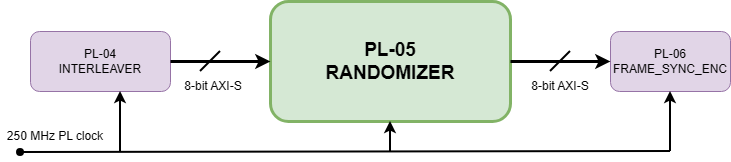
\includegraphics[width=0.85\linewidth]{figures/ch4/ch4_pl05_pipeline}
  \caption{Pipeline position of PL-05 \texttt{randomizer} in the J.83B
           Annex~B transmit chain.}
  \label{fig:pl05_pipeline}
\end{figure}

% ------------------------------------------------------------------
% §2  INTERFACE
% ------------------------------------------------------------------

\paragraph{Interface.}

Figure~\ref{fig:pl05_ip_block} shows the \texttt{randomizer} core as
packaged in Vivado \ac{ip} Integrator.
The \texttt{s\_axi} slave group on the left receives the interleaved
byte stream from PL-04; the \texttt{m\_axi} master group on the right
drives PL-06.
The simplicity of the block reflects the module's streaming-only design:
no additional control ports, sub-module instances, or configuration
registers appear.
The port list is given in Table~\ref{tab:pl05_ports}.

% [ALT: Screenshot of the randomizer IP core in Vivado IP Integrator.
%       The block is labeled randomizer with the subtitle J.83B Randomizer
%       (PL-05) (Pre-Production). On the left side the s_axi slave
%       interface group shows ports s_axi_tdata[7:0], s_axi_tvalid, and
%       s_axi_tready. Control ports clk and rst_n appear below. On the
%       right side the m_axi master interface group shows ports
%       m_axi_tdata[7:0], m_axi_tvalid, and m_axi_tready. No other ports
%       or sub-blocks are visible.]
\begin{figure}[htbp]
  \centering
  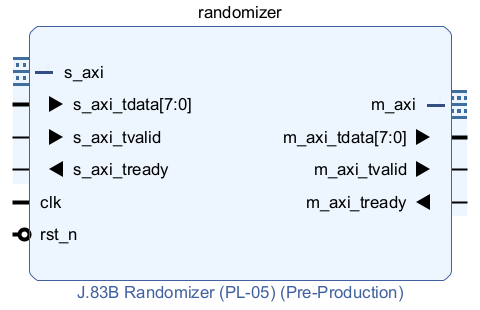
\includegraphics[width=0.55\linewidth]{figures/ch4/ch4_pl05_ip_block}
  \caption{PL-05 \texttt{randomizer} packaged as a Vivado \ac{ip} core in
           \ac{ip} Integrator, showing the \texttt{s\_axi} slave and
           \texttt{m\_axi} master interface groups.}
  \label{fig:pl05_ip_block}
\end{figure}

\FloatBarrier

\begin{table}[htbp]
  \caption{PL-05 \texttt{randomizer} port list.}
  \label{tab:pl05_ports}
  \centering
  \small
  \begin{tabular}{llcp{2.7cm}p{5.8cm}}
    \hline
    Port                    & Dir  & Width & Protocol               & Description \\
    \hline
    \texttt{clk}            & in   & 1     & Clock                  & 250\,MHz \ac{pl} fabric clock \\[2pt]
    \texttt{rst\_n}         & in   & 1     & Reset                  & Synchronous active-low \\[2pt]
    \texttt{s\_axi\_tdata}  & in   & 8     & \ac{axi}4-Stream slave & Interleaved byte from PL-04; bit~7 always 0 \\[2pt]
    \texttt{s\_axi\_tvalid} & in   & 1     & \ac{axi}4-Stream slave & Upstream data valid \\[2pt]
    \texttt{s\_axi\_tready} & out  & 1     & \ac{axi}4-Stream slave & Direct wire: \texttt{= m\_axi\_tready} \\[2pt]
    \texttt{m\_axi\_tdata}  & out  & 8     & \ac{axi}4-Stream master & Randomized byte to PL-06; bit~7 always 0 \\[2pt]
    \texttt{m\_axi\_tvalid} & out  & 1     & \ac{axi}4-Stream master & Direct wire: \texttt{= s\_axi\_tvalid} \\[2pt]
    \texttt{m\_axi\_tready} & in   & 1     & \ac{axi}4-Stream master & Downstream backpressure \\
    \hline
  \end{tabular}
\end{table}

% ------------------------------------------------------------------
% §3  STREAMING OPERATION
% ------------------------------------------------------------------

\paragraph{Streaming Operation.}

PL-05 has no \ac{fsm}, no operating phases, and no initialisation window.
All output signals are combinational functions of the current inputs and
the \ac{pn} sequence counter \texttt{sym\_cnt}.
The module is ready to accept and produce data the cycle after
\texttt{rst\_n} is released — there is no delay comparable to PL-04's
8{,}128-cycle \ac{bram} init window.

The core operation is a single bitwise XOR applied to every accepted
symbol:

\begin{equation}
  \mathtt{m\_axi\_tdata} =
  \left\{
    \texttt{1'b0},\;
    \mathtt{s\_axi\_tdata}[6:0] \oplus
    \mathtt{rseq\_rom}[\mathtt{sym\_cnt}]
  \right\}
  \label{eq:randomizer_xor}
\end{equation}

\noindent where \texttt{rseq\_rom[sym\_cnt]} is the precomputed
\ac{gf}(128) \ac{pn} sequence entry at the current symbol position.
Bit~7 of the output is hardwired to \texttt{1'b0}; all arithmetic
operates on the 7-bit symbol field.

The counter \texttt{sym\_cnt} advances by~1 on every input handshake,
cycling from~0 to~11{,}263 and wrapping to~0~\cite{ITU_J83}.
During downstream stalls or upstream valid gaps (such as the 5-cycle
Horner stall from PL-03), \texttt{sym\_cnt} freezes: no symbol is
accepted, no counter step occurs, and the \ac{pn} sequence position is
preserved exactly.
Backpressure propagates as a direct wire in both directions:
\texttt{s\_axi\_tready} is tied to \texttt{m\_axi\_tready} with no
gating, and \texttt{m\_axi\_tvalid} mirrors \texttt{s\_axi\_tvalid} with
zero latency.

Table~\ref{tab:pl05_signals} summarises all output signal assignments,
which apply uniformly at all times after reset.

\begin{table}[htbp]
  \caption{PL-05 output signal assignments (all times after reset).}
  \label{tab:pl05_signals}
  \centering
  \small
  \begin{tabular}{p{3.0cm}p{6.0cm}lp{3.0cm}}
    \hline
    Signal                       & Value                                                          & Type          & Notes \\
    \hline
    \texttt{s\_axi\_tready}      & \texttt{m\_axi\_tready}                                        & Direct wire   & No gating; no init window \\[2pt]
    \texttt{m\_axi\_tvalid}      & \texttt{s\_axi\_tvalid}                                        & Direct wire   & Zero-latency mirror \\[2pt]
    \texttt{m\_axi\_tdata[7]}    & \texttt{1'b0}                                                  & Constant      & Bit~7 always zero \\[2pt]
    \texttt{m\_axi\_tdata[6:0]}  & \texttt{s\_tdata[6:0]}~$\oplus$~\texttt{rseq\_rom[sym\_cnt]}  & Combinational & Core \ac{pn} XOR \\
    \hline
  \end{tabular}
\end{table}

% ------------------------------------------------------------------
% §4  MEMORY RESOURCES
% ------------------------------------------------------------------

\paragraph{Memory Resources.}

The \ac{pn} sequence is stored as a 11{,}264-entry, 7-bit-wide
read-only table \texttt{RSEQ\_ROM}, synthesized entirely as distributed
\ac{lut} logic.
The \texttt{rom\_style = "distributed"} synthesis attribute, combined with
an asynchronous (unregistered) read port, causes Vivado to infer
combinational \ac{lut} logic rather than \ac{lut}-\ac{ram} or
\ac{bram}.
Post-implementation confirms no \ac{bram} and no \ac{lut} as memory
usage: the 11{,}264 entries are fully decoded by a MUXF7/MUXF8 cascade
(644 and 322 cells respectively).
The \ac{rom} content was pre-computed offline using the ANSpect J.83B
reference implementation~\cite{ITU_J83}, with \texttt{write\_rseq\_rom.m}
generating the $\mathrm{GF}(128)$ \ac{pn} sequence and writing it to
\texttt{rseq\_rom.mem}.
Table~\ref{tab:pl05_rom} lists the \ac{rom} parameters.

\begin{table}[htbp]
  \caption{PL-05 \texttt{RSEQ\_ROM} configuration.}
  \label{tab:pl05_rom}
  \centering
  \small
  \begin{tabular}{p{3.5cm}p{11.5cm}}
    \hline
    Parameter              & Value \\
    \hline
    Depth $\times$ Width   & $11{,}264 \times 7$~bits (78{,}848~bits total) \\[2pt]
    Content                & $\mathrm{GF}(128)$ \ac{pn} sequence,
                             $f(x) = x^3 + x + \alpha^3$,
                             $p(x) = x^7 + x^3 + 1$,
                             initial state $c_2 = c_1 = c_0 = \texttt{0x7F}$ \\[2pt]
    Period                 & 11{,}264 symbols ($88 \times 128$, 256-QAM mode)~\cite{ITU_J83} \\[2pt]
    Synthesis              & Distributed \ac{lut} logic + MUXF7/MUXF8; NOT \ac{bram}, NOT \ac{lut}-RAM \\[2pt]
    Address                & \texttt{sym\_cnt[13:0]} (14-bit, combinational read) \\[2pt]
    Source file            & \texttt{rseq\_rom.mem} \\[2pt]
    Generator              & \texttt{write\_rseq\_rom.m} via ANSpect J.83B reference implementation \\[2pt]
    Verification           & 11{,}264/11{,}264 entries confirmed \\
    \hline
  \end{tabular}
\end{table}

% ------------------------------------------------------------------
% §5  RTL ARCHITECTURE
% ------------------------------------------------------------------

\paragraph{RTL Architecture.}
% [FIGURE OMITTED: datapath diagram figures/ch4_pl05_datapath — omitted by author]

With the streaming operation and memory resources established, this section
describes their hardware realization.

\textit{sym\_cnt counter.}
The only registered element is the 14-bit counter \texttt{sym\_cnt[13:0]},
implemented as 14~logical flip-flops in the \ac{rtl}.
Because \texttt{sym\_cnt} addresses all 11{,}264 entries of
\texttt{RSEQ\_ROM}, each bit drives 1{,}358~\acp{lut}, producing a
high-fanout net on every counter bit.
Vivado automatically replicates \texttt{sym\_cnt} approximately 3.9 times
during implementation, yielding 54~\texttt{FDRE} primitives in the placed
netlist, to distribute the load across slices without routing congestion.
No \ac{rtl} change was required; the replication is a synthesis artifact.
The resulting critical timing path at 250\,MHz is route-dominated:
\texttt{sym\_cnt\_reg\_rep[13]} $\to$ LUT3 $\to$ LUT6 $\to$ \ac{ff}
reset pin, with 89.1\% of the 2.565\,ns total data delay attributable
to routing, yielding a worst negative slack of $+1.236$\,ns and an
estimated $F_{\max}$ of approximately 361.8\,MHz.

\textit{XOR datapath and output assignments.}
The XOR of \texttt{s\_axi\_tdata[6:0]} and \texttt{rseq\_rom[sym\_cnt]}
is purely combinational, resolving in the same clock cycle as the input.
Bit~7 of the output is hardwired to \texttt{1'b0} via the
\texttt{\{1'b0, ...\}} concatenation, preserving the 7-bit symbol
constraint imposed by PL-03~\cite{ITU_J83}.
\texttt{s\_axi\_tready} and \texttt{m\_axi\_tvalid} are single
\texttt{assign} statements with no logic gates — direct electrical
connections.

\textit{Combinational output boundary.}
\texttt{m\_axi\_tdata} is combinational: the output resolves in the same
cycle as input with zero pipeline latency.
This design means the combinational path from PL-04's \ac{bram} output
through PL-05's XOR gate continues into PL-06's input, crossing two
module boundaries without a registered cut.
Standalone timing at 250\,MHz closed with $+1.236$\,ns margin.
System-level functional correctness through the PL-04$\to$PL-05$\to$PL-06
boundary was confirmed in integration simulation and on board~\cite{PYNQ_DOC}.

\FloatBarrier

% ------------------------------------------------------------------
% §6  INTERFACE CONTRACT
% ------------------------------------------------------------------

\paragraph{Interface Contract.}

\textit{Upstream (\texttt{s\_axi\_*}, from PL-04 interleaver):}
\begin{itemize}
  \item Input bytes carry 7-bit interleaved symbols with bit~7 guaranteed
        zero by PL-03/PL-04; this property is preserved
        throughout~\cite{ITU_J83}.
  \item \texttt{s\_axi\_tready} is a direct wire to \texttt{m\_axi\_tready}
        with no gating.
        Unlike PL-04, there is no initialisation window — the module is
        ready to accept data the cycle after \texttt{rst\_n} is released.
  \item Upstream must hold \texttt{s\_axi\_tvalid} and \texttt{s\_axi\_tdata}
        stable whenever \texttt{s\_axi\_tready}~$= 0$~\cite{ARM_IHI0022}.
        PL-04 satisfies this through its own emit-phase buffering.
  \item PL-03 Horner stall gaps (\texttt{tvalid}~$= 0$, 5~cycles) pass
        through PL-04 to PL-05.
        \texttt{sym\_cnt} freezes during these gaps; no symbol is skipped
        or duplicated.
  \item No \texttt{tlast} signal is used.
\end{itemize}

\textit{Downstream (\texttt{m\_axi\_*}, to PL-06 frame sync encoder):}
\begin{itemize}
  \item One randomized byte is emitted per accepted input byte.
        Bit~7 is always zero.
  \item Zero pipeline latency: \texttt{m\_axi\_tdata} is valid in the
        same cycle as the input handshake.
        Downstream must sample on the rising clock edge when
        \texttt{m\_axi\_tvalid} and \texttt{m\_axi\_tready} are both
        asserted simultaneously.
  \item \texttt{m\_axi\_tvalid} is a direct wire to \texttt{s\_axi\_tvalid}.
        During upstream valid gaps, \texttt{m\_axi\_tvalid}~$= 0$ and
        \texttt{m\_axi\_tdata} is undefined; downstream must not sample
        during these periods.
  \item If upstream drives \texttt{s\_axi\_tvalid}~$= 1$ while
        \texttt{rst\_n}~$= 0$, \texttt{m\_axi\_tvalid}~$= 1$ may assert.
        \texttt{sym\_cnt} does not advance during reset.
        Downstream PL-06 must gate sampling on \texttt{rst\_n}.
  \item Backpressure is fully propagated:
        \texttt{m\_axi\_tready}~$= 0$ stalls upstream immediately via
        the direct \texttt{s\_axi\_tready} wire~\cite{ARM_IHI0022}.
  \item No \texttt{tlast} signal is generated.
\end{itemize}

\FloatBarrier

% ------------------------------------------------------------------
% §7  RESOURCE UTILIZATION AND TIMING
% ------------------------------------------------------------------

\paragraph{Resource Utilization and Timing.}
\leavevmode\par
\begin{table}[!h]
  \caption{PL-05 post-implementation resource utilization
           (\texttt{xczu48dr-ffvg1517-2-e}, speed-grade~$-2$
           PRODUCTION, Vivado~2024.2, 19~Jul~2026).}
  \label{tab:pl05_resources}
  \centering
  \begin{tabular}{lrrl}
    \hline
    Resource     & Used    & Available  & Utilization \\
    \hline
    \ac{lut6}    & 1{,}358 & 425{,}280  & 0.32\%      \\[2pt]
    \ac{ff}      &      54 & 850{,}560  & $<0.01$\%   \\[2pt]
    MUXF7        &     644 & N/A        & N/A          \\[2pt]
    MUXF8        &     322 & N/A        & N/A          \\[2pt]
    \ac{bram}    &       0 & 1{,}080    & 0.00\%      \\[2pt]
    \ac{dsp}     &       0 & 4{,}272    & 0.00\%      \\[2pt]
    UltraRAM     &       0 & 80         & 0.00\%      \\
    \hline
  \end{tabular}
\end{table}

\begin{table}[!h]
  \caption{PL-05 post-implementation timing summary
           (\texttt{xczu48dr-ffvg1517-2-e}, speed-grade~$-2$
           PRODUCTION, Vivado~2024.2, 19~Jul~2026).}
  \label{tab:pl05_timing}
  \centering
  \begin{tabular}{lll}
    \hline
    Metric                   & 250\,MHz             & 100\,MHz           \\
    \hline
    WNS, setup               & $+1.236$\,ns (MET)   & $+5.365$\,ns (MET) \\[2pt]
    WHS, hold                & $+0.060$\,ns (MET)   & $+0.065$\,ns (MET) \\[2pt]
    Est.\ $F_{\max}$         & $\approx 361.8$\,MHz & $\approx 216$\,MHz  \\[2pt]
    Failing endpoints        & 0                    & 0                  \\
    \hline
  \end{tabular}
\end{table}

\FloatBarrier

% ------------------------------------------------------------------
% §8  VERIFICATION
% ------------------------------------------------------------------

\paragraph{Verification.}

\textit{Simulation.}
Unit-level verification confirmed the XOR datapath against hand-traced
\ac{gf}(128) \ac{pn} sequence values at selected offsets, a full
11{,}264-entry range sweep confirming all values in the range
\texttt{0x00}--\texttt{0x7F}, and the self-inverse property — applying
the XOR twice with the same \texttt{sym\_cnt} offset recovers the
original input exactly.
The 45{,}056-byte golden vector sweep was run at full rate, under 30\%
output backpressure, with 20\% input gaps, and under combined input
and output throttling, confirming bit-exact agreement in all four
conditions.
Counter behavior was verified across all boundary conditions: freeze
during \texttt{tready}~$= 0$ and \texttt{tvalid}~$= 0$ stalls, wrap
from 11{,}263 to~0, mid-stream reset returning \texttt{sym\_cnt} to~0,
and counter hold throughout a reset with \texttt{tvalid}~$= 1$ asserted.
Seven \ac{axi}4-Stream \ac{sva} checks — including direct-wire
verification of \texttt{s\_tready}~$=$~\texttt{m\_tready} and
\texttt{m\_tvalid}~$=$~\texttt{s\_tvalid}, bit~7 zero invariant, and
counter-gate correctness — fired zero violations across all 60 checks.

Integration testing in the PL-02$\to$PL-06 chain confirmed \ac{pn}
sequence wrap from position~11{,}263 to~0 at the chain level, correct
passthrough of PL-03 Horner stall gaps with no \texttt{sym\_cnt}
advancement, and 8{,}304/8{,}304 trellis groups bit-exact across all
throttle, backpressure, reset, and data pattern scenarios.

\textit{Hardware.}

\begin{table}[htbp]
  \caption{PL-05 hardware validation summary.}
  \label{tab:pl05_hw}
  \centering
  \small
  \begin{tabular}{p{3.2cm}lp{4.5cm}p{3.2cm}l}
    \hline
    Bitfile & Clock & Method & Result & Date \\
    \hline
    \path{pl_2_6.bit}\\(PL-02$\to$PL-06 chain)
      & 100\,MHz
      & PYNQ \ac{dma} loopback~\cite{PYNQ_DOC}; output compared
        to \path{stage5_framesync_bits.bin}
      & 8{,}304/8{,}304 groups bit-exact; \ac{pn} sequence correctness
        confirmed
      & 28-Jul-2026 \\
    \hline
  \end{tabular}
\end{table}

Board validation of PL-05 was performed indirectly as part of the
PL-02$\to$PL-06 transmit chain.
Bit-exact agreement at the PL-06 output across 8{,}304 trellis groups
confirms correct \ac{pn} sequence generation, XOR application, bit~7
suppression, and counter wrap behavior.
The bitfile was evaluated at 100\,MHz; production operation targets
250\,MHz, confirmed by post-implementation timing at
$F_{\max} \approx 361.8$\,MHz~(Table~\ref{tab:pl05_timing}).

%\clearpage

% ============================================================
% CH-4.3.6  PL-06: FRAME_SYNC_ENC
% Source : PL-06_FRAME_SYNC_ENC_handoff.md v2.2  27-Jul-2026
%          frame_sync_enc.sv v2.2
%          PL-11_anspect_ctrl_regs_handoff.md v2.0 (ctrl_word source)
% NDA CLEAR: IMPL [4.3] — received
% Preflight : CH-4.3.6 [PL-06] — PASS  22-Oct-2026
%   IMG-1 [x]  IMG-2 [x]  IMG-3 [OMITTED — author]  IMG-4 [x]  IMG-5 [x]
% Expanded  : 22-Oct-2026
% Template  : CARRY_FORWARD.md §1–§8 v1.2
%   Structure: §3 FSM → §4 RTL Architecture
%   Memory Resources: N/A — trailer constants are localparams; no ROM/BRAM
% ============================================================

\subsection{PL-06: Frame Sync Encoder}
\label{subsec:pl06}

% ------------------------------------------------------------------
% §1  OVERVIEW
% ------------------------------------------------------------------

The frame sync encoder module (PL-06) implements the J.83B Annex~B frame
synchronisation stage specified in \S\,B.5.3 of the standard~\cite{ITU_J83}.
It serializes the 11{,}264 randomized 7-bit symbols of one \ac{fec} frame into
a continuous bit stream, appends the 40-bit frame sync trailer, and packs the
result into 2{,}076 consecutive 38-bit trellis groups for the trellis encoder
(PL-07).
The algorithmic background — frame arithmetic, trailer structure, and trellis
group boundaries — is presented in Section~\ref{sec:framesync}; this section
covers its hardware realization.
The module is hand-coded SystemVerilog (\texttt{frame\_sync\_enc.sv},
revision~v2.2), operates as an \ac{axi}4-Stream slave-to-master pair at
the 250\,MHz \ac{pl} fabric clock, and carries a testbench status of
TB-PASS (43/43 checks, 0 failures).

Figure~\ref{fig:pl06_pipeline} shows the pipeline position of PL-06.
Unlike PL-02 through PL-05, which carry byte-wide symbol streams on an
8-bit bus, PL-06 changes the bus width: the 8-bit input from PL-05 carries
one 7-bit symbol per transfer, while the 40-bit output delivers 38-bit
trellis groups to PL-07.
PL-11 (\texttt{anspect\_ctrl\_regs}), shown above PL-06 in the figure,
supplies a 4-bit \texttt{ctrl\_word} sideband from its
\texttt{FRAME\_SYNC\_CW} register at \ac{axi}4-Lite offset~\texttt{0x20};
this value is embedded as the upper nibble of the fifth trailer byte and
must be written by the processing system before the TX chain is enabled.

% [ALT: Block diagram. Top row: PL-11 anspect_ctrl_regs block with a
%       labeled 4-bit ctrl_word arrow pointing down to PL-06. Main row
%       (left to right): PL-05 RANDOMIZER connected by 8-bit AXI-S arrow
%       to PL-06 FRAME_SYNC_ENC (highlighted green), connected by 40-bit
%       AXI-S arrow to PL-07 TRELLIS_ENC. A 250 MHz PL clock label
%       appears at the lower left; no CDC markers at any boundary.]
\begin{figure}[htbp]
  \centering
  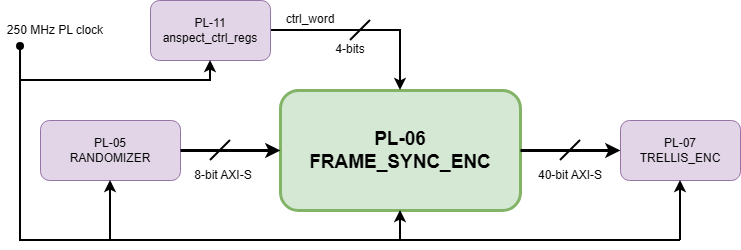
\includegraphics[width=0.88\linewidth]{figures/ch4/ch4_pl06_pipeline}
  \caption{Pipeline position of PL-06 \texttt{frame\_sync\_enc}.
           The \texttt{ctrl\_word[3:0]} sideband is driven from PL-11
           \texttt{anspect\_ctrl\_regs} (\texttt{FRAME\_SYNC\_CW},
           \ac{axi}4-Lite offset~\texttt{0x20}).}
  \label{fig:pl06_pipeline}
\end{figure}

% ------------------------------------------------------------------
% §2  INTERFACE
% ------------------------------------------------------------------

\paragraph{Interface.}

Figure~\ref{fig:pl06_ip_block} shows the packaged core in Vivado \ac{ip}
Integrator.
Compared to PL-02 through PL-05, two additional ports are visible:
\texttt{ctrl\_word[3:0]} on the left side receives the frame sync control
word from PL-11, and \texttt{m\_axi\_tlast} on the right side carries the
frame boundary signal to PL-07.
The port list is given in Table~\ref{tab:pl06_ports}.

% [ALT: Screenshot of the frame_sync_enc IP core in Vivado IP Integrator.
%       The block is labeled frame_sync_enc with subtitle J.83B Frame Sync
%       Encoder (PL-06) (Pre-Production). On the left: s_axi slave group
%       with s_axi_tdata[7:0], s_axi_tvalid, s_axi_tready; control ports
%       clk, rst_n; and ctrl_word[3:0]. On the right: m_axi master group
%       with m_axi_tdata[39:0], m_axi_tlast, m_axi_tvalid, m_axi_tready.]
\begin{figure}[htbp]
  \centering
  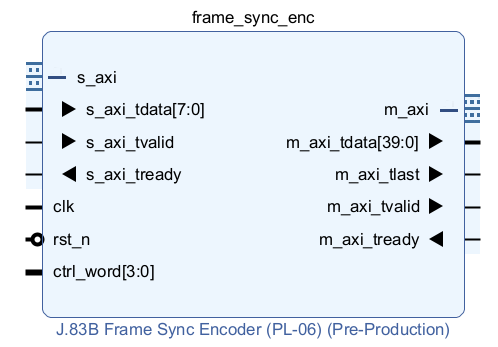
\includegraphics[width=0.58\linewidth]{figures/ch4/ch4_pl06_ip_block}
  \caption{PL-06 \texttt{frame\_sync\_enc} packaged as a Vivado \ac{ip}
           core in \ac{ip} Integrator, showing the \texttt{s\_axi} slave,
           \texttt{m\_axi} master, \texttt{ctrl\_word[3:0]} sideband, and
           \texttt{m\_axi\_tlast} ports.}
  \label{fig:pl06_ip_block}
\end{figure}

\FloatBarrier

\begin{table}[htbp]
  \caption{PL-06 \texttt{frame\_sync\_enc} port list.}
  \label{tab:pl06_ports}
  \centering
  \small
  \begin{tabular}{llcp{2.7cm}p{5.8cm}}
    \hline
    Port                    & Dir  & Width & Protocol               & Description \\
    \hline
    \texttt{clk}            & in   & 1     & Clock                  & 250\,MHz \ac{pl} fabric clock \\[2pt]
    \texttt{rst\_n}         & in   & 1     & Reset                  & Synchronous active-low \\[2pt]
    \texttt{ctrl\_word}     & in   & 4     & Sideband               & Interleaver depth ctrl word from PL-11; quasi-static \\[2pt]
    \texttt{s\_axi\_tdata}  & in   & 8     & \ac{axi}4-Stream slave & 7-bit randomized symbol from PL-05; bit~7 always 0 \\[2pt]
    \texttt{s\_axi\_tvalid} & in   & 1     & \ac{axi}4-Stream slave & Upstream data valid \\[2pt]
    \texttt{s\_axi\_tready} & out  & 1     & \ac{axi}4-Stream slave & State-dependent; pulses every 7~clocks in DATA \\[2pt]
    \texttt{m\_axi\_tdata}  & out  & 40    & \ac{axi}4-Stream master & 38-bit trellis group to PL-07; bits~[39:38]~$=$~\texttt{2'b00} \\[2pt]
    \texttt{m\_axi\_tvalid} & out  & 1     & \ac{axi}4-Stream master & Downstream data valid; registered \\[2pt]
    \texttt{m\_axi\_tready} & in   & 1     & \ac{axi}4-Stream master & Downstream backpressure \\[2pt]
    \texttt{m\_axi\_tlast}  & out  & 1     & \ac{axi}4-Stream master & Frame boundary; asserted on group~2{,}075 only \\
    \hline
  \end{tabular}
\end{table}

% ------------------------------------------------------------------
% §3  FSM
% ------------------------------------------------------------------

\paragraph{FSM.}

PL-06 processes one \ac{fec} frame at a time through a fixed three-stage
sequence: wait, serialize, emit trailer.
Figure~\ref{fig:pl06_fsm} shows the state diagram with the three states
arranged in a clockwise cycle, each corresponding directly to one of these tasks.

% [ALT: State diagram with three circular states arranged clockwise.
%       IDLE(0) top-left: s_tready=pipe_en, m_tvalid=out_valid. DATA(1)
%       top-right: s_tready=(bit_cnt==6) and pipe_en and (sym_cnt!=11264),
%       m_tvalid=out_valid. TRAILER(2) bottom-centre: s_tready=0 hard,
%       m_tvalid=out_valid. A dashed reset arc enters IDLE. IDLE to DATA:
%       input_handshake. DATA to TRAILER: sym_cnt==11264 and bit_cnt==6
%       and pipe_en. TRAILER to IDLE: trailer_cnt==39 and grp_done.
%       Default to IDLE (synthesis safety).]
\begin{figure}[htbp]
  \centering
  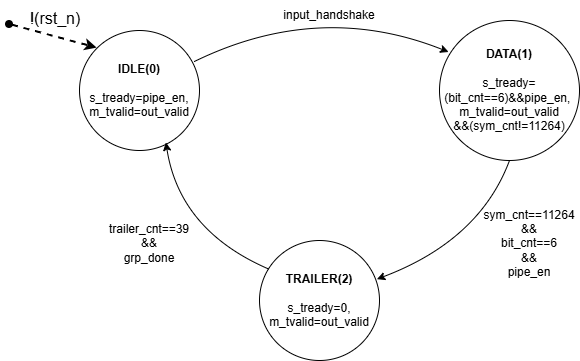
\includegraphics[width=0.70\linewidth]{figures/ch4/ch4_pl06_fsm}
  \caption{PL-06 \ac{fsm} state transition diagram.
           \texttt{input\_hs}: \texttt{s\_axi\_tvalid \&\ s\_axi\_tready};
           \texttt{grp\_done}: \texttt{accum\_cnt}~$= 37$ and
           \texttt{accum\_en}.
           One-hot synthesis: IDLE state \ac{ff} is \texttt{FDSE}
           (synchronous set on reset).}
  \label{fig:pl06_fsm}
\end{figure}

\FloatBarrier

\texttt{IDLE} is the reset state.
\texttt{out\_valid} is low after a frame boundary reset, so \texttt{pipe\_en}
asserts and \texttt{s\_axi\_tready} is driven high.
The first input handshake from PL-05 latches the first symbol and transitions
the module to \texttt{DATA}.

\texttt{DATA} is the main serialization loop.
The module accepts one 7-bit symbol every 7~clock cycles: the accepted symbol
is latched into \texttt{sym\_reg} and its 7~bits are shifted \ac{msb}-first
into the 38-bit accumulator at one bit per clock.
\texttt{s\_axi\_tready} asserts only at \texttt{bit\_cnt}~$= 6$, creating
a 1:7 upstream duty cycle — PL-05 is granted one transfer window every
7~clocks.
Every 38 accumulated bits, \texttt{grp\_done} fires and the completed
38-bit group is latched into \texttt{out\_reg} with \texttt{out\_valid}
set, making it available to PL-07.
This continues for all 11{,}264 symbols.
When the last bit of the 11{,}264th symbol is serialized
(\texttt{sym\_cnt}~$= 11{,}264$, \texttt{bit\_cnt}~$= 6$),
\texttt{last\_sym\_last\_bit} triggers and the module transitions to
\texttt{TRAILER}.

\texttt{TRAILER} emits the 40-bit J.83B frame sync trailer~\cite{ITU_J83}.
\texttt{s\_axi\_tready} is hard-deasserted for the entire trailer window,
blocking upstream PL-05 for approximately 40~clock cycles.
The same 38-bit accumulator continues uninterrupted — only the bit source
changes from \texttt{sym\_reg} to the combinational trailer \ac{lut}
indexed by \texttt{trailer\_cnt[5:0]}.
The 40~trailer bits complete group~2{,}074 (36 data bits already in the
accumulator are joined by the first 2 trailer bits) and fill
group~2{,}075 (38 trailer bits exclusively).
When \texttt{trailer\_cnt}~$= 39$ and \texttt{grp\_done} fires,
group~2{,}075 is latched with \texttt{out\_tlast}~$= 1$,
all counters reset, and the module returns to \texttt{IDLE}.

Table~\ref{tab:pl06_fsm} gives the handshake signal values per state.
\texttt{pipe\_en} asserts when no group is pending (\texttt{out\_valid}~$= 0$)
or when the pending group is being consumed (\texttt{output\_handshake}),
and gates all datapath advances.

\begin{table}[htbp]
  \caption{PL-06 \ac{fsm} state summary.}
  \label{tab:pl06_fsm}
  \centering
  \small
  \begin{tabular}{lp{4.0cm}lp{6.5cm}}
    \hline
    State             & \texttt{s\_axi\_tready}      & \texttt{m\_axi\_tvalid} & Task \\
    \hline
    \texttt{IDLE}     & \texttt{pipe\_en}             & \texttt{out\_valid}
                      & Awaiting first symbol; output pipeline may still be draining \\[4pt]
    \texttt{DATA}     & \texttt{bit\_cnt}~$= 6$,
                        \texttt{pipe\_en},
                        \texttt{sym\_cnt}~$\neq 11{,}264$
                      & \texttt{out\_valid}
                      & Serializing 11{,}264 symbols into 38-bit groups at 1:7 input duty cycle \\[4pt]
    \texttt{TRAILER}  & \texttt{0} (hard)
                      & \texttt{out\_valid}
                      & Emitting 40-bit frame sync trailer; upstream fully blocked \\
    \hline
  \end{tabular}
\end{table}

% ------------------------------------------------------------------
% §4  RTL ARCHITECTURE
% ------------------------------------------------------------------
% Memory Resources: N/A — trailer bytes synthesised as localparams;
%                  no ROM files, no BRAM, no $readmemh required.

\paragraph{RTL Architecture.}
% [FIGURE OMITTED: datapath diagram figures/ch4_pl06_datapath — omitted by author]

With the \ac{fsm} established, this section describes how each state's
task is realized in hardware.

\textit{Accumulator pipeline.}
The 38-bit shift register \texttt{accum[37:0]} accepts one bit per clock
when \texttt{accum\_en} asserts:
$\mathtt{accum} \leftarrow \{\mathtt{accum}[36:0],\,\mathtt{current\_bit}\}$.
A companion counter \texttt{accum\_cnt[5:0]} tracks the number of bits
written; when \texttt{accum\_cnt}~$= 37$ and \texttt{accum\_en} fire
simultaneously, \texttt{grp\_done} pulses.
On \texttt{grp\_done}, \texttt{out\_reg} latches the completed 38-bit
group, \texttt{accum} and \texttt{accum\_cnt} reset to zero, and
\texttt{out\_valid} is set.
This pipeline is shared between \texttt{DATA} and \texttt{TRAILER} — only
the source of \texttt{current\_bit} changes between states.

\textit{Bit serializer.}
In \texttt{DATA}, \texttt{current\_bit} is driven by the bit serializer:
$\mathtt{data\_bit} = \mathtt{sym\_reg}[6 - \mathtt{bit\_cnt}]$, emitting
\texttt{sym\_reg[6]} (\ac{msb}) first.
The \texttt{bit\_cnt} counter advances when \texttt{bit\_shift\_en}
asserts, wrapping from~6 to~0 on each accepted symbol.
A correctness requirement governs this wrap: when \texttt{bit\_cnt}~$= 6$
and \texttt{s\_axi\_tvalid}~$= 0$, both \texttt{bit\_shift\_en} and
\texttt{accum\_en} are suppressed to hold the serializer and accumulator
frozen until a valid symbol arrives.
Without this suppression, a valid-low gap at \texttt{bit\_cnt}~$= 6$
would wrap the counter and shift stale \texttt{sym\_reg} content into
the accumulator, misaligning \texttt{accum\_cnt} at the
\texttt{DATA}$\to$\texttt{TRAILER} boundary and making the terminal
condition of \texttt{TRAILER} unreachable.
For the final symbol (\texttt{sym\_cnt}~$= 11{,}264$), the suppression
is bypassed: once the 11{,}264th input handshake has occurred,
\texttt{s\_axi\_tready}~$= 0$ prevents any further upstream transfer and
\texttt{s\_axi\_tvalid} is irrelevant; the final symbol's 7-clock
serialization window must complete unconditionally.

\textit{Trailer source.}
In \texttt{TRAILER}, \texttt{current\_bit} is driven by a combinational
\ac{lut} indexed by \texttt{trailer\_cnt[5:0]}.
The 40~trailer bits are organized as four fixed sync bytes
(\texttt{0x71}, \texttt{0xE8}, \texttt{0x4D}, \texttt{0xD4}),
the 4-bit \texttt{ctrl\_word} at positions 32--35 (\ac{msb} first), and
four reserved zero bits at positions 36--39~\cite{ITU_J83}.
The fixed bytes are defined as localparams and constant-folded into
\ac{lut} logic by Vivado at synthesis — no \ac{rom} files, no \ac{bram},
and no \texttt{\$readmemh} are required.
\texttt{ctrl\_word} is read combinationally with no pipeline register; a
write to \texttt{FRAME\_SYNC\_CW} (PL-11, \ac{axi}4-Lite
offset~\texttt{0x20}) takes effect within the same clock cycle the write
completes.

\textit{Output register.}
\texttt{out\_reg}, \texttt{out\_valid}, and \texttt{out\_tlast} are all
registered on \texttt{grp\_done}, providing a registered cut between the
accumulator and the \ac{axi}4-Stream output.
\texttt{m\_axi\_tdata}~$=$ \texttt{\{2'b00, out\_reg\}}: bits~[39:38]
are permanently zero-padded to satisfy the \ac{axi}4-Stream requirement
that \texttt{TDATA} width be a multiple of~8 bits~\cite{ARM_IHI0022}; the effective 38-bit
trellis group occupies bits~[37:0].
\texttt{m\_axi\_tlast}~$=$ \texttt{out\_tlast \&\ out\_valid} ensures the
frame boundary signal can never assert without a valid transfer.

\FloatBarrier

% ------------------------------------------------------------------
% §5  INTERFACE CONTRACT
% ------------------------------------------------------------------

\paragraph{Interface Contract.}

\textit{Upstream (\texttt{s\_axi\_*}, from PL-05 randomizer):}
\begin{itemize}
  \item Input bytes carry 7-bit randomized symbols; bit~7 is always zero
        and is truncated internally via
        \texttt{s\_tdata[6:0]}~\cite{ITU_J83}.
  \item \texttt{s\_axi\_tready} asserts for exactly one clock every
        7~cycles in \texttt{DATA}.
        PL-05 must hold \texttt{s\_axi\_tvalid} and \texttt{s\_axi\_tdata}
        stable during the 6~cycles when \texttt{s\_tready}~$= 0$~\cite{ARM_IHI0022}.
  \item Upstream valid gaps (including the 5-cycle Horner stall from
        PL-03) arriving at \texttt{bit\_cnt}~$= 6$ are handled by the
        serializer freeze: the bit counter and accumulator hold state
        until a valid symbol is present, with no data loss or
        \ac{pn} counter skip in PL-05.
  \item \texttt{s\_axi\_tready}~$= 0$ for the full \texttt{TRAILER}
        phase (approximately 40~clock cycles); PL-05 holds its output
        stable throughout.
  \item No \texttt{tlast} signal is used.
\end{itemize}

\textit{Downstream (\texttt{m\_axi\_*} and \texttt{m\_axi\_tlast}, to
PL-07 trellis encoder):}
\begin{itemize}
  \item Exactly 2{,}076 trellis groups are emitted per \ac{fec} frame,
        carried in \texttt{m\_axi\_tdata[37:0]}.
        Bits~[39:38] are permanently zero.
  \item \texttt{m\_axi\_tdata} is registered and remains stable while
        \texttt{m\_axi\_tvalid}~$= 1$ and
        \texttt{m\_axi\_tready}~$= 0$~\cite{ARM_IHI0022}.
  \item \texttt{m\_axi\_tlast} is asserted on group~2{,}075 only —
        exactly once per \ac{fec} frame.
        PL-07 uses \texttt{tlast} to detect the frame boundary without
        a sideband group counter.
  \item \texttt{m\_axi\_tlast} is gated by \texttt{out\_valid} and
        can never assert without a simultaneous valid transfer.
  \item No further \texttt{tlast} is generated until the following frame's
        group~2{,}075.
\end{itemize}

Figure~\ref{fig:pl06_packet} shows the complete output frame structure.
The yellow non-sync region covers groups~0 through~2{,}070 — 2{,}071
groups assembled entirely from serialized symbol data during the
\texttt{DATA} state.
The pink sync region covers groups~2{,}071 through~2{,}074, where the frame
data nears its end and the trailer begins entering the accumulator;
group~2{,}074 carries 36~data bits alongside the first 2~trailer bits at
the \texttt{DATA}$\to$\texttt{TRAILER} boundary.
The green final sync group is group~2{,}075, carrying the remaining
38~trailer bits exclusively and the only group on which
\texttt{m\_axi\_tlast} asserts.
The bit-packing inset in the figure confirms that
\texttt{m\_axi\_tdata[39:38]~=~2'b00} is padding and
\texttt{m\_axi\_tdata[37:0]} carries the 38-bit trellis group \ac{msb}-first
from the output register.

% [ALT: Diagram of one FEC frame on the 40-bit AXI-Stream output bus,
%       labeled 2076 x 40-bit transfers. Yellow section labeled non-sync
%       groups[0..2070] with 2071 symbols showing Group-0 through
%       Group-2070. Pink section labeled sync groups[0..3] with 4
%       symbols showing Group-0 through Group-3. Green section labeled
%       final sync with 1 symbol showing Group-0. Below: tlast asserted
%       on group 2075 (final sync group) only; TRAILER phase upstream
%       blocked s_tready=0 for ~40 cycles at end; ctrl_word embedded in
%       group 2075 trailer bits. An inset table shows bit packing:
%       bit[39:38]=2'b00 padding; bit[37:0]=38-bit trellis group MSB-first
%       from PL-06 accumulator.]
\begin{figure}[htbp]
  \centering
  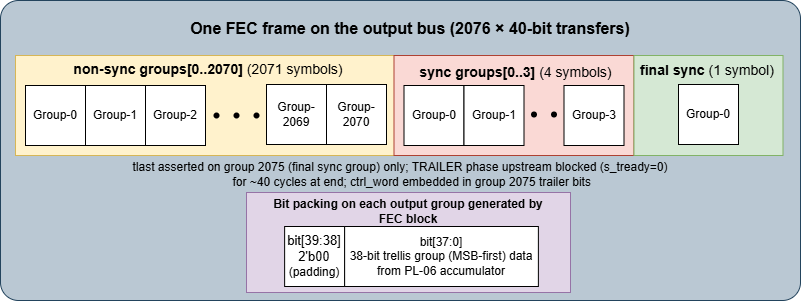
\includegraphics[width=0.90\linewidth]{figures/ch4/ch4_pl06_packet}
  \caption{PL-06 output frame structure: one \ac{fec} frame on the
           downstream 40-bit \ac{axi}4-Stream bus.
           2{,}076 groups total; \texttt{m\_axi\_tlast} asserted on
           group~2{,}075 only; \texttt{s\_axi\_tready}~$= 0$ during
           the approximately 40-cycle \texttt{TRAILER}
           phase~\cite{ITU_J83}.}
  \label{fig:pl06_packet}
\end{figure}

\FloatBarrier

% ------------------------------------------------------------------
% §6  RESOURCE UTILIZATION AND TIMING
% ------------------------------------------------------------------

\paragraph{Resource Utilization and Timing.}
\leavevmode\par
\begin{table}[!h]
  \caption{PL-06 post-implementation resource utilization
           (\texttt{xczu48dr-ffvg1517-2-e}, speed-grade~$-2$
           PRODUCTION, Vivado~2024.2, 22~Oct~2026).}
  \label{tab:pl06_resources}
  \centering
  \begin{tabular}{lrrl}
    \hline
    Resource     & Used  & Available  & Utilization \\
    \hline
    LUT          &   42  & 425{,}280  & $<0.01$\%   \\[2pt]
    \ac{ff}      &  116  & 850{,}560  & 0.01\%      \\[2pt]
    CARRY8       &    2  & N/A        & N/A          \\[2pt]
    \ac{bram}    &    0  & 1{,}080    & 0.00\%      \\[2pt]
    \ac{dsp}     &    0  & 4{,}272    & 0.00\%      \\[2pt]
    UltraRAM     &    0  & 80         & 0.00\%      \\
    \hline
  \end{tabular}
\end{table}

\begin{table}[!h]
  \caption{PL-06 post-implementation timing summary
           (\texttt{xczu48dr-ffvg1517-2-e}, speed-grade~$-2$
           PRODUCTION, Vivado~2024.2, 22~Oct~2026).}
  \label{tab:pl06_timing}
  \centering
  \begin{tabular}{lll}
    \hline
    Metric                   & 250\,MHz             & 100\,MHz           \\
    \hline
    WNS, setup               & $+2.263$\,ns (MET)   & $+7.954$\,ns (MET) \\[2pt]
    WHS, hold                & $+0.042$\,ns (MET)   & $+0.036$\,ns (MET) \\[2pt]
    Est.\ $F_{\max}$         & $\approx 576$\,MHz   & $\approx 489$\,MHz  \\[2pt]
    Failing endpoints        & 0                    & 0                  \\
    \hline
  \end{tabular}
\end{table}

\FloatBarrier

% ------------------------------------------------------------------
% §7  VERIFICATION
% ------------------------------------------------------------------

\paragraph{Verification.}

\textit{Simulation.}
Unit-level verification used a golden vector sweep of 4~\ac{fec} frames
(8{,}304 trellis groups) against the MATLAB reference model
\texttt{j83b\_frame\_sync\_enc.m}, confirming bit-exact agreement across
all groups including the trailer boundary at group~2{,}074 and the
\texttt{tlast}-marked group~2{,}075.
A \texttt{ctrl\_word} sweep over values \texttt{0x0}, \texttt{0x5},
\texttt{0xA}, and \texttt{0xF} confirmed correct trailer byte~4 encoding
in all cases.
\texttt{m\_axi\_tlast} was confirmed to assert exactly once per frame on
group~2{,}075.
Reset recovery was verified in both the \texttt{DATA} and \texttt{TRAILER}
states with full golden output recovery.
The 1:7 upstream duty cycle and \texttt{TRAILER}-phase upstream blocking
behavior were confirmed under all backpressure and throttle combinations.
All \ac{axi}4-Stream \ac{sva} checks fired zero violations.

Integration testing in the PL-02$\to$PL-06 chain confirmed
8{,}304/8{,}304 trellis groups bit-exact against the stage~5 golden
reference, a deterministic frame period of 88{,}584 cycles across all
4~frames with zero variance, a \texttt{TRAILER} duration of exactly
40~cycles per frame, and correct handling of all PL-03 Horner stall
gaps arriving at \texttt{bit\_cnt}~$= 6$.
All 126 integration checks passed with zero \ac{sva} fires.

\textit{Hardware.}

\begin{table}[htbp]
  \caption{PL-06 hardware validation summary.}
  \label{tab:pl06_hw}
  \centering
  \small
  \begin{tabular}{p{3.2cm}lp{4.5cm}p{3.2cm}l}
    \hline
    Bitfile & Clock & Method & Result & Date \\
    \hline
    \path{pl_2_6.bit}\\(PL-02$\to$PL-06 chain)
      & 100\,MHz
      & PYNQ \ac{dma} loopback~\cite{PYNQ_DOC}; output compared
        to \path{stage5_framesync_bits.bin}
      & 8{,}304/8{,}304 groups bit-exact; all 4 frames;
        \texttt{ctrl\_word}~$= 0$ confirmed end-to-end
      & 28-Jul-2026 \\
    \hline
  \end{tabular}
\end{table}

Board validation of PL-06 was performed as the output stage of the
PL-02$\to$PL-06 transmit chain, confirming correct symbol serialization,
trailer insertion, group packing, and \texttt{tlast} generation at the
hardware level.
Trailer group~2{,}074 bits~[1:0]~$=$ \texttt{0b01} and
group~2{,}075~$=$ \texttt{0x31E84DD400} were verified across all
4~\ac{fec} frames.
The bitfile was evaluated at 100\,MHz; production operation targets
250\,MHz, confirmed by post-implementation timing at
$F_{\max} \approx 576$\,MHz~(Table~\ref{tab:pl06_timing}).

\clearpage

\subsection{PL-07: Trellis Encoder}
\label{subsec:pl07}
% [NDA-IMPL] — BLOCKED
% TODO: Requires NDA CLEAR: IMPL [4.3.7] + handoff for PL-07

\subsection{PL-08: QAM-256 Mapper}
\label{subsec:pl08}
% [NDA-IMPL] — BLOCKED
% TODO: Requires NDA CLEAR: IMPL [4.3.8] + handoff for PL-08

\subsection{PL-09: SRRC FIR TX}
\label{subsec:pl09}
% [NDA-IMPL] — BLOCKED
% TODO: Requires NDA CLEAR: IMPL [4.3.9] + handoff for PL-09

\subsection{PL-10: SD-FEC LDPC}
\label{subsec:pl10}
% [NDA-IMPL] — BLOCKED
% [NDA-ALGO] — LDPC interaction with O-EMA overlay
%              PERMANENTLY BLOCKED — never draftable
% TODO: Structural existence may be acknowledged only
%   - Internal algorithm: hard block, do not draft or paraphrase
%   - Requires NDA CLEAR: IMPL [4.3.10] for structural frame only

\subsection{PL-11: Register File RTL}
\label{subsec:pl11}
% [NDA-IMPL] — BLOCKED
% TODO: Requires NDA CLEAR: IMPL [4.3.11] + handoff for PL-11
%   - AXI-Lite register map is NDA-IMPL — do not include offsets
%     or field definitions without explicit clearance

\subsection{PL-12: IQ Combiner}
\label{subsec:pl12}
% [NDA-IMPL] — BLOCKED
% TODO: Requires NDA CLEAR: IMPL [4.3.12] + handoff for PL-12
\clearpage  
% ------------------------------------------------------------
\section{Programmable Logic: RX Chain}
\label{sec:pl_rx}
% [NDA-IMPL] — BLOCKED
% TODO: Section intro requires NDA CLEAR: IMPL [4.4] + handoff
%   - PL-13 through PL-23 — one subsection each

\subsection{PL-13: SRRC FIR RX}
\label{subsec:pl13}
% [NDA-IMPL] — BLOCKED
% TODO: Requires NDA CLEAR: IMPL [4.4.1] + handoff for PL-13

\subsection{PL-14: Symbol Timing Recovery}
\label{subsec:pl14}
% [NDA-IMPL] — BLOCKED
% TODO: Requires NDA CLEAR: IMPL [4.4.2] + handoff for PL-14

\subsection{PL-15: Carrier and Phase Recovery}
\label{subsec:pl15}
% [NDA-IMPL] — BLOCKED
% TODO: Requires NDA CLEAR: IMPL [4.4.3] + handoff for PL-15

\subsection{PL-16: QAM-256 Demapper}
\label{subsec:pl16}
% [NDA-IMPL] — BLOCKED
% TODO: Requires NDA CLEAR: IMPL [4.4.4] + handoff for PL-16

\subsection{PL-17: Trellis Decoder}
\label{subsec:pl17}
% [NDA-IMPL] — BLOCKED
% TODO: Requires NDA CLEAR: IMPL [4.4.5] + handoff for PL-17

\subsection{PL-18: Frame Sync Detection}
\label{subsec:pl18}
% [NDA-IMPL] — BLOCKED
% TODO: Requires NDA CLEAR: IMPL [4.4.6] + handoff for PL-18

\subsection{PL-19: De-Randomizer}
\label{subsec:pl19}
% [NDA-IMPL] — BLOCKED
% TODO: Requires NDA CLEAR: IMPL [4.4.7] + handoff for PL-19

\subsection{PL-20: De-Interleaver}
\label{subsec:pl20}
% [NDA-IMPL] — BLOCKED
% TODO: Requires NDA CLEAR: IMPL [4.4.8] + handoff for PL-20

\subsection{PL-21: Reed-Solomon Decoder}
\label{subsec:pl21}
% [NDA-IMPL] — BLOCKED
% TODO: Requires NDA CLEAR: IMPL [4.4.9] + handoff for PL-21

\subsection{PL-22: Transport Framing RX}
\label{subsec:pl22}
% [NDA-IMPL] — BLOCKED
% TODO: Requires NDA CLEAR: IMPL [4.4.10] + handoff for PL-22

\subsection{PL-23: AXI DMA S2MM}
\label{subsec:pl23}
% [NDA-IMPL] — BLOCKED
% TODO: Requires NDA CLEAR: IMPL [4.4.11] + handoff for PL-23
\clearpage  
% ------------------------------------------------------------
\section{RF Data Converter}
\label{sec:rfdc}
% [NDA-IMPL] — BLOCKED
% TODO: Section intro requires NDA CLEAR: IMPL [4.5] + handoff
%   - Existence of RFDC block may be stated (public IP)
%   - Tile configuration parameters: NDA-IMPL — no detail without clearance

\subsection{DAC: Tile 228}
\label{subsec:dac_tile228}
% [NDA-IMPL] — BLOCKED (RFDC-01)
% TODO: Requires NDA CLEAR: IMPL [4.5.1] + handoff
%   - Tile/channel configuration: NDA-IMPL
%   - NCO, interpolation settings: NDA-IMPL

\subsection{ADC: Tile 224}
\label{subsec:adc_tile224}
% [NDA-IMPL] — BLOCKED (RFDC-02)
% TODO: Requires NDA CLEAR: IMPL [4.5.2] + handoff
%   - Tile/channel configuration: NDA-IMPL
\clearpage  
% ------------------------------------------------------------
\section{RF Front-End}
\label{sec:rf_frontend}
% [NDA-IMPL] — BLOCKED
% TODO: Section intro requires NDA CLEAR: IMPL [4.6] + handoff

\subsection{TX Path}
\label{subsec:rf_tx}
% [NDA-IMPL] — BLOCKED (RF-01)
% TODO: Requires NDA CLEAR: IMPL [4.6.1] + handoff
%   - DAC balun + SMA TX path

\subsection{RX Path}
\label{subsec:rf_rx}
% [NDA-IMPL] — BLOCKED (RF-02)
% TODO: Requires NDA CLEAR: IMPL [4.6.2] + handoff
%   - ADC balun + SMA RX path
\clearpage  
% ------------------------------------------------------------
\section{Clocking Subsystem}
\label{sec:clocking}
% [NDA-IMPL] — BLOCKED
% TODO: Section intro requires NDA CLEAR: IMPL [4.7] + handoff
%   - Clock chip existence may be stated (public component)
%   - Register settings: NDA-IMPL — no detail without clearance

\subsection{LMK04828}
\label{subsec:lmk04828}
% [NDA-IMPL] — BLOCKED (EXT-01)
% TODO: Requires NDA CLEAR: IMPL [4.7.1] + handoff
%   - Clock distribution chip — register configuration: NDA-IMPL

\subsection{LMX2594}
\label{subsec:lmx2594}
% [NDA-IMPL] — BLOCKED (EXT-02)
% TODO: Requires NDA CLEAR: IMPL [4.7.2] + handoff
%   - PLL/VCO chip — register configuration: NDA-IMPL

\subsection{xrfclk API}
\label{subsec:xrfclk}
% [NDA-IMPL] — BLOCKED (EXT-03)
% TODO: Requires NDA CLEAR: IMPL [4.7.3] + handoff
%   - Xilinx xrfclk Python API — usage detail: NDA-IMPL
\clearpage  
% ------------------------------------------------------------
\section{Test and Measurement}
\label{sec:test_measurement}
% STATUS: OPEN — all subsections freely draftable from public specs
% TODO: Section intro paragraph
%   - Overview of test setup: source → DUT → sink + spectrum
%   - Loopback topology description

\subsection{H-Thunder-1 Reference Signal}
\label{subsec:hthunder}
% STATUS: OPEN — public product spec
% TODO:
%   - H-Thunder-1 J.83B / 256-QAM reference signal generator
%   - Role: known-good J.83B signal source for RX validation
%   - Public product specification detail
%   - Cite product datasheet \cite{NEEDED} % [CITE NEEDED]

\subsection{HDHomeRun: Source and Sink}
\label{subsec:hdhomerun}
% STATUS: OPEN — public product (EXT-04, EXT-05)
% TODO:
%   - HDHomeRun \#1 role: MPEG-TS source over GigE (TX path input)
%   - HDHomeRun \#2 role: MPEG-TS sink over GigE (RX path output)
%   - Public product — cite product page \cite{NEEDED} % [CITE NEEDED]

\subsection{Spectrum Analysis}
\label{subsec:spectrum_analysis}
% STATUS: OPEN — general methodology
% TODO:
%   - Spectrum analyzer role in RF output validation
%   - Measurements performed: channel power, spectral shape,
%     occupied bandwidth, noise floor
%   - General methodology — no proprietary test vector data
\clearpage  
% ------------------------------------------------------------
\section{Verification and Results}
\label{sec:verification}
% [NDA-IMPL] — BLOCKED
% TODO: Section intro requires NDA CLEAR: IMPL [4.9] + handoff
%   - Stage map existence may be referenced (public README portion)
%   - Test vector details: NDA-IMPL

\subsection{Test Vectors}
\label{subsec:test_vectors}
% [NDA-IMPL] — BLOCKED (partially public stage map only)
% TODO: Requires NDA CLEAR: IMPL [4.9.1] + handoff
%   - Stage boundary file names (public): stage0–stage8
%   - File formats (public): uint8 / int16 per stage
%   - Internal content and mismatch analysis: NDA-IMPL

\subsection{Loopback Validation}
\label{subsec:loopback}
% [NDA-IMPL] — BLOCKED
% TODO: Requires NDA CLEAR: IMPL [4.9.2] + handoff
%   - Loopback path topology (structural) may be described after clearance
%   - BER / EVM / verification results: NDA-IMPL
